\documentclass[nooutcomes]{ximera}


\graphicspath{
  {./}
  {1-1QuantitativeReasoning/}
  {1-2RelationsAndGraphs/}
  {1-3ChangingInTandem/}
  {2-1LinearEquations/}
  {2-2LinearModeling/}
  {2-3ExponentialModeling/}
  {3-1WhatIsAFunction/}
  {3-2FunctionProperties/}
  {3-3AverageRatesOfChange/}
  {4-1BuildingNewFunctions/}
  {4-2Polynomials/}
  {5-1RationalFunctions/}
   {5-2ExponentialFunctions/}
  {6-1Domain/}
  {6-2Range/}
  {6-3CompositionOfFunctions/}
  {7-1ZerosOfFunctions/}
  {7-XZerosOfPolynomials/}
  {7-2ZerosOfFamousFunctions/}
  {8-0Review/}
  {8-1FunctionTransformations/}
  {8-2SolvingInequalities/}
  {8-3FunctionTransformationsProject/}
  {9-1RightTriangleTrig/}
  {9-2TheUnitCircle/}
  {9-3TrigIdentities/}
  {10-1UnitCircleToFunctionGraph/}
  {10-2TrigFunctions/}
  {10-3SomeApplicationsOfTrig/}
  {11-1InverseFunctionsRevisited/}
  {11-2Logarithms/}
  {11-3InverseTrig/}
  {12-1SystemsOfEquations/}
  {12-2NonlinearSystems/}
  {12-3ApplicationsOfSystems/}
  {13-1SecantLinesRevisited/}
  {13-2Functions-TheBigPicture/}
  {14-1DisplacementVsDistance/}
  {1-1QuantitativeReasoning/exercises/}
  {1-2RelationsAndGraphs/exercises/}
  {../1-3ChangingInTandem/exercises/}
  {../2-1LinearEquations/exercises/}
  {../2-2LinearModeling/exercises/}
  {../2-3ExponentialModeling/exercises/}
  {../3-1WhatIsAFunction/exercises/}
  {../3-2FunctionProperties/exercises/}
  {../3-3AverageRatesOfChange/exercises/}
  {../5-2ExponentialFunctions/exercises/}
  {../4-1BuildingNewFunctions/exercises/}
  {../4-2Polynomials/exercises/}
  {../5-1RationalFunctions/exercises/}
  {../6-1Domain/exercises/}
  {../6-2Range/exercises/}
  {../6-3CompositionOfFunctions/exercises/}
  {../7-1ZerosOfFunctions/exercises/}
  {../7-XZerosOfPolynomials/exercises/}
  {../7-2ZerosOfFamousFunctions/exercises/}
  {../8-1FunctionTransformations/exercises/}
  {../12-1SystemsOfEquations/exercises/}
  {../8-3FunctionTransformationsProject/exercises/}
  {../8-0Review/exercises/}
  {../8-2SolvingInequalities/exercises/}
  {../8-3FunctionTransformationsProject/exercises/}
  {../9-1RightTriangleTrig/exercises/}
  {../9-2TheUnitCircle/exercises/}
  {../9-3TrigIdentities/exercises/}
  {../10-1UnitCircleToFunctionGraph/exercises/}
  {../10-2TrigFunctions/exercises/}
  {../10-3SomeApplicationsOfTrig/exercises/}
  {../11-1InverseFunctionsRevisited/exercises/}
  {../11-2Logarithms/exercises/}
  {../11-3InverseTrig/exercises/}
  {../12-1SystemsOfEquations/exercises/}
  {../12-2NonlinearSystems/exercises/}
  {../12-3ApplicationsOfSystems/exercises/}
  {../13-1SecantLinesRevisited/exercises/}
  {../13-2Functions-TheBigPicture/exercises/}
  {../14-1DisplacementVsDistance/exercises/}
}

\DeclareGraphicsExtensions{.pdf,.png,.jpg,.eps}

\newcommand{\mooculus}{\textsf{\textbf{MOOC}\textnormal{\textsf{ULUS}}}}

\usepackage[makeroom]{cancel} %% for strike outs

\ifxake
\else
\usepackage[most]{tcolorbox}
\fi


%\typeout{************************************************}
%\typeout{New Environments}
%\typeout{************************************************}

%% to fix for web can be removed when deployed offically with ximera2
\let\image\relax\let\endimage\relax
\NewEnviron{image}{% 
  \begin{center}\BODY\end{center}% center
}



\NewEnviron{folder}{
      \addcontentsline{toc}{section}{\textbf{\BODY}}
}

\ifxake
\let\summary\relax
\let\endsummary\relax
\newtheorem*{summary}{Summary}
\newtheorem*{callout}{Callout}
\newtheorem*{overview}{Overview}
\newtheorem*{objectives}{Objectives}
\newtheorem*{motivatingQuestions}{Motivating Questions}
\newtheorem*{MM}{Metacognitive Moment}
      
%% NEEDED FOR XIMERA 2
%\ximerizedEnvironment{summary}
%\ximerizedEnvironment{callout}
%\ximerizedEnvironment{overview} 
%\ximerizedEnvironment{objectives}
%\ximerizedEnvironment{motivatingQuestions}
%\ximerizedEnvironment{MM}
\else
%% CALLOUT
\NewEnviron{callout}{
  \begin{tcolorbox}[colback=blue!5, breakable,pad at break*=1mm]
      \BODY
  \end{tcolorbox}
}
%% MOTIVATING QUESTIONS
\NewEnviron{motivatingQuestions}{
  \begin{tcolorbox}[ breakable,pad at break*=1mm]
    \textbf{\Large Motivating Questions}\hfill
    %\begin{itemize}[label=\textbullet]
      \BODY
    %\end{itemize}
  \end{tcolorbox}
}
%% OBJECTIVES
\NewEnviron{objectives}{  
    \vspace{.5in}
      %\begin{tcolorbox}[colback=orange!5, breakable,pad at break*=1mm]
    \textbf{\Large Learning Objectives}
    \begin{itemize}[label=\textbullet]
      \BODY
    \end{itemize}
    %\end{tcolorbox}
}
%% DEFINITION
\let\definition\relax
\let\enddefinition\relax
\NewEnviron{definition}{
  \begin{tcolorbox}[ breakable,pad at break*=1mm]
    \noindent\textbf{Definition}~
      \BODY
  \end{tcolorbox}
}
%% OVERVIEW
\let\overview\relax
\let\overview\relax
\NewEnviron{overview}{
  \begin{tcolorbox}[ breakable,pad at break*=1mm]
    \textbf{\Large Overview}
    %\begin{itemize}[label=\textbullet] %% breaks Xake
      \BODY
    %\end{itemize}
  \end{tcolorbox}
}
%% SUMMARY
\let\summary\relax
\let\endsummary\relax
\NewEnviron{summary}{
  \begin{tcolorbox}[ breakable,pad at break*=1mm]
    \textbf{\Large Summary}
    %\begin{itemize}[label=\textbullet] %% breaks Xake
      \BODY
    %\end{itemize}
  \end{tcolorbox}
}
%% REMARK
\let\remark\relax
\let\endremark\relax
\NewEnviron{remark}{
  \begin{tcolorbox}[colback=green!5, breakable,pad at break*=1mm]
    \noindent\textbf{Remark}~
      \BODY
  \end{tcolorbox}
}
%% EXPLANATION
\let\explanation\relax
\let\endexplanation\relax
\NewEnviron{explanation}{
    \normalfont
    \noindent\textbf{Explanation}~
      \BODY
}
%% EXPLORATION
\let\exploration\relax
\let\endexploration\relax
\NewEnviron{exploration}{
  \begin{tcolorbox}[colback=yellow!10, breakable,pad at break*=1mm]
    \noindent\textbf{Exploration}~
      \BODY
  \end{tcolorbox}
}
%% METACOGNITIVE MOMENTS
\let\MM\relax
\let\endMM\relax
\NewEnviron{MM}{
  \begin{tcolorbox}[colback=pink!15, breakable,pad at break*=1mm]
    \noindent\textbf{Metacognitive Moment}~
      \BODY
  \end{tcolorbox}
}


\fi





%Notes on what envirnoment to use:  Example with Explanation in text; if they are supposed to answer- Problem; no answer - Exploration


%\typeout{************************************************}
%% Header and footers
%\typeout{************************************************}

\newcommand{\licenseAcknowledgement}{Licensed under Creative Commons 4.0}
\newcommand{\licenseAPC}{\renewcommand{\licenseAcknowledgement}{\textbf{Acknowledgements:} Active Prelude to Calculus (https://activecalculus.org/prelude) }}
\newcommand{\licenseSZ}{\renewcommand{\licenseAcknowledgement}{\textbf{Acknowledgements:} Stitz Zeager Open Source Mathematics (https://www.stitz-zeager.com/) }}
\newcommand{\licenseAPCSZ}{\renewcommand{\licenseAcknowledgement}{\textbf{Acknowledgements:} Active Prelude to Calculus (https://activecalculus.org/prelude) and Stitz Zeager Open Source Mathematics (https://www.stitz-zeager.com/) }}
\newcommand{\licenseORCCA}{\renewcommand{\licenseAcknowledgement}{\textbf{Acknowledgements:}Original source material, products with readable and accessible
math content, and other information freely available at pcc.edu/orcca.}}
\newcommand{\licenseY}{\renewcommand{\licenseAcknowledgement}{\textbf{Acknowledgements:} Yoshiwara Books (https://yoshiwarabooks.org/)}}
\newcommand{\licenseOS}{\renewcommand{\licenseAcknowledgement}{\textbf{Acknowledgements:} OpenStax College Algebra (https://openstax.org/details/books/college-algebra)}}
\newcommand{\licenseAPCSZCSCC}{\renewcommand{\licenseAcknowledgement}{\textbf{Acknowledgements:} Active Prelude to Calculus (https://activecalculus.org/prelude), Stitz Zeager Open Source Mathematics (https://www.stitz-zeager.com/), CSCC PreCalculus and Calculus texts (https://ximera.osu.edu/csccmathematics)}}

\ifxake\else %% do nothing on the website
\usepackage{fancyhdr}
\pagestyle{fancy}
\fancyhf{}
\fancyhead[R]{\sectionmark}
\fancyfoot[L]{\thepage}
\fancyfoot[C]{\licenseAcknowledgement}
\renewcommand{\headrulewidth}{0pt}
\renewcommand{\footrulewidth}{0pt}
\fi

%%%%%%%%%%%%%%%%



%\typeout{************************************************}
%\typeout{Table of Contents}
%\typeout{************************************************}


%% Edit this to change the font style
\newcommand{\sectionHeadStyle}{\sffamily\bfseries}


\makeatletter

%% part uses arabic numerals
\renewcommand*\thepart{\arabic{part}}


\ifxake\else
\renewcommand\chapterstyle{%
  \def\maketitle{%
    \addtocounter{titlenumber}{1}%
    \pagestyle{fancy}
    \phantomsection
    \addcontentsline{toc}{section}{\textbf{\thepart.\thetitlenumber\hspace{1em}\@title}}%
                    {\flushleft\small\sectionHeadStyle\@pretitle\par\vspace{-1.5em}}%
                    {\flushleft\LARGE\sectionHeadStyle\thepart.\thetitlenumber\hspace{1em}\@title \par }%
                    {\setcounter{problem}{0}\setcounter{sectiontitlenumber}{0}}%
                    \par}}





\renewcommand\sectionstyle{%
  \def\maketitle{%
    \addtocounter{sectiontitlenumber}{1}
    \pagestyle{fancy}
    \phantomsection
    \addcontentsline{toc}{subsection}{\thepart.\thetitlenumber.\thesectiontitlenumber\hspace{1em}\@title}%
    {\flushleft\small\sectionHeadStyle\@pretitle\par\vspace{-1.5em}}%
    {\flushleft\Large\sectionHeadStyle\thepart.\thetitlenumber.\thesectiontitlenumber\hspace{1em}\@title \par}%
    %{\setcounter{subsectiontitlenumber}{0}}%
    \par}}



\renewcommand\section{\@startsection{paragraph}{10}{\z@}%
                                     {-3.25ex\@plus -1ex \@minus -.2ex}%
                                     {1.5ex \@plus .2ex}%
                                     {\normalfont\large\sectionHeadStyle}}
\renewcommand\subsection{\@startsection{subparagraph}{10}{\z@}%
                                    {3.25ex \@plus1ex \@minus.2ex}%
                                    {-1em}%
                                    {\normalfont\normalsize\sectionHeadStyle}}

\fi

%% redefine Part
\renewcommand\part{%
   {\setcounter{titlenumber}{0}}
  \if@openright
    \cleardoublepage
  \else
    \clearpage
  \fi
  \thispagestyle{plain}%
  \if@twocolumn
    \onecolumn
    \@tempswatrue
  \else
    \@tempswafalse
  \fi
  \null\vfil
  \secdef\@part\@spart}

\def\@part[#1]#2{%
    \ifnum \c@secnumdepth >-2\relax
      \refstepcounter{part}%
      \addcontentsline{toc}{part}{\thepart\hspace{1em}#1}%
    \else
      \addcontentsline{toc}{part}{#1}%
    \fi
    \markboth{}{}%
    {\centering
     \interlinepenalty \@M
     \normalfont
     \ifnum \c@secnumdepth >-2\relax
       \huge\sffamily\bfseries \partname\nobreakspace\thepart
       \par
       \vskip 20\p@
     \fi
     \Huge \bfseries #2\par}%
    \@endpart}
\def\@spart#1{%
    {\centering
     \interlinepenalty \@M
     \normalfont
     \Huge \bfseries #1\par}%
    \@endpart}
\def\@endpart{\vfil\newpage
              \if@twoside
               \if@openright
                \null
                \thispagestyle{empty}%
                \newpage
               \fi
              \fi
              \if@tempswa
                \twocolumn
                \fi}



\makeatother





%\typeout{************************************************}
%\typeout{Stuff from Ximera}
%\typeout{************************************************}



\usepackage{array}  %% This is for typesetting long division
\setlength{\extrarowheight}{+.1cm}
\newdimen\digitwidth
\settowidth\digitwidth{9}
\def\divrule#1#2{
\noalign{\moveright#1\digitwidth
\vbox{\hrule width#2\digitwidth}}}





\newcommand{\RR}{\mathbb R}
\newcommand{\R}{\mathbb R}
\newcommand{\N}{\mathbb N}
\newcommand{\Z}{\mathbb Z}

\newcommand{\sagemath}{\textsf{SageMath}}


\def\d{\,d}
%\renewcommand{\d}{\mathop{}\!d}
\newcommand{\dd}[2][]{\frac{\d #1}{\d #2}}
\newcommand{\pp}[2][]{\frac{\partial #1}{\partial #2}}
\renewcommand{\l}{\ell}
\newcommand{\ddx}{\frac{d}{\d x}}



%\newcommand{\unit}{\,\mathrm}
\newcommand{\unit}{\mathop{}\!\mathrm}
\newcommand{\eval}[1]{\bigg[ #1 \bigg]}
\newcommand{\seq}[1]{\left( #1 \right)}
\renewcommand{\epsilon}{\varepsilon}
\renewcommand{\phi}{\varphi}


\renewcommand{\iff}{\Leftrightarrow}

\DeclareMathOperator{\arccot}{arccot}
\DeclareMathOperator{\arcsec}{arcsec}
\DeclareMathOperator{\arccsc}{arccsc}
\DeclareMathOperator{\sign}{sign}


%\DeclareMathOperator{\divergence}{divergence}
%\DeclareMathOperator{\curl}[1]{\grad\cross #1}
\newcommand{\lto}{\mathop{\longrightarrow\,}\limits}

\renewcommand{\bar}{\overline}

\colorlet{textColor}{black}
\colorlet{background}{white}
\colorlet{penColor}{blue!50!black} % Color of a curve in a plot
\colorlet{penColor2}{red!50!black}% Color of a curve in a plot
\colorlet{penColor3}{red!50!blue} % Color of a curve in a plot
\colorlet{penColor4}{green!50!black} % Color of a curve in a plot
\colorlet{penColor5}{orange!80!black} % Color of a curve in a plot
\colorlet{penColor6}{yellow!70!black} % Color of a curve in a plot
\colorlet{fill1}{penColor!20} % Color of fill in a plot
\colorlet{fill2}{penColor2!20} % Color of fill in a plot
\colorlet{fillp}{fill1} % Color of positive area
\colorlet{filln}{penColor2!20} % Color of negative area
\colorlet{fill3}{penColor3!20} % Fill
\colorlet{fill4}{penColor4!20} % Fill
\colorlet{fill5}{penColor5!20} % Fill
\colorlet{gridColor}{gray!50} % Color of grid in a plot

\newcommand{\surfaceColor}{violet}
\newcommand{\surfaceColorTwo}{redyellow}
\newcommand{\sliceColor}{greenyellow}




\pgfmathdeclarefunction{gauss}{2}{% gives gaussian
  \pgfmathparse{1/(#2*sqrt(2*pi))*exp(-((x-#1)^2)/(2*#2^2))}%
}





%\typeout{************************************************}
%\typeout{ORCCA Preamble.Tex}
%\typeout{************************************************}


%% \usepackage{geometry}
%% \geometry{letterpaper,total={408pt,9.0in}}
%% Custom Page Layout Adjustments (use latex.geometry)
%% \usepackage{amsmath,amssymb}
%% \usepackage{pgfplots}
\usepackage{pifont}                                         %needed for symbols, s.a. airplane symbol
\usetikzlibrary{positioning,fit,backgrounds}                %needed for nested diagrams
\usetikzlibrary{calc,trees,positioning,arrows,fit,shapes}   %needed for set diagrams
\usetikzlibrary{decorations.text}                           %needed for text following a curve
\usetikzlibrary{arrows,arrows.meta}                         %needed for open/closed intervals
\usetikzlibrary{positioning,3d,shapes.geometric}            %needed for 3d number sets tower

%% NEEDED FOR XIMERA 1
%\usetkzobj{all}       %NO LONGER VALID
%%%%%%%%%%%%%%

\usepackage{tikz-3dplot}
\usepackage{tkz-euclide}                     %needed for triangle diagrams
\usepgfplotslibrary{fillbetween}                            %shade regions of a plot
\usetikzlibrary{shadows}                                    %function diagrams
\usetikzlibrary{positioning}                                %function diagrams
\usetikzlibrary{shapes}                                     %function diagrams
%%% global colors from https://www.pcc.edu/web-services/style-guide/basics/color/ %%%
\definecolor{ruby}{HTML}{9E0C0F}
\definecolor{turquoise}{HTML}{008099}
\definecolor{emerald}{HTML}{1c8464}
\definecolor{amber}{HTML}{c7502a}
\definecolor{amethyst}{HTML}{70485b}
\definecolor{sapphire}{HTML}{263c53}
\colorlet{firstcolor}{sapphire}
\colorlet{secondcolor}{turquoise}
\colorlet{thirdcolor}{emerald}
\colorlet{fourthcolor}{amber}
\colorlet{fifthcolor}{amethyst}
\colorlet{sixthcolor}{ruby}
\colorlet{highlightcolor}{green!50!black}
\colorlet{graphbackground}{white}
\colorlet{wood}{brown!60!white}
%%% curve, dot, and graph custom styles %%%
\pgfplotsset{firstcurve/.style      = {color=firstcolor,  mark=none, line width=1pt, {Kite}-{Kite}, solid}}
\pgfplotsset{secondcurve/.style     = {color=secondcolor, mark=none, line width=1pt, {Kite}-{Kite}, solid}}
\pgfplotsset{thirdcurve/.style      = {color=thirdcolor,  mark=none, line width=1pt, {Kite}-{Kite}, solid}}
\pgfplotsset{fourthcurve/.style     = {color=fourthcolor, mark=none, line width=1pt, {Kite}-{Kite}, solid}}
\pgfplotsset{fifthcurve/.style      = {color=fifthcolor,  mark=none, line width=1pt, {Kite}-{Kite}, solid}}
\pgfplotsset{highlightcurve/.style  = {color=highlightcolor,  mark=none, line width=5pt, -, opacity=0.3}}   % thick, opaque curve for highlighting
\pgfplotsset{asymptote/.style       = {color=gray, mark=none, line width=1pt, <->, dashed}}
\pgfplotsset{symmetryaxis/.style    = {color=gray, mark=none, line width=1pt, <->, dashed}}
\pgfplotsset{guideline/.style       = {color=gray, mark=none, line width=1pt, -}}
\tikzset{guideline/.style           = {color=gray, mark=none, line width=1pt, -}}
\pgfplotsset{altitude/.style        = {dashed, color=gray, thick, mark=none, -}}
\tikzset{altitude/.style            = {dashed, color=gray, thick, mark=none, -}}
\pgfplotsset{radius/.style          = {dashed, thick, mark=none, -}}
\tikzset{radius/.style              = {dashed, thick, mark=none, -}}
\pgfplotsset{rightangle/.style      = {color=gray, mark=none, -}}
\tikzset{rightangle/.style          = {color=gray, mark=none, -}}
\pgfplotsset{closedboundary/.style  = {color=black, mark=none, line width=1pt, {Kite}-{Kite},solid}}
\tikzset{closedboundary/.style      = {color=black, mark=none, line width=1pt, {Kite}-{Kite},solid}}
\pgfplotsset{openboundary/.style    = {color=black, mark=none, line width=1pt, {Kite}-{Kite},dashed}}
\tikzset{openboundary/.style        = {color=black, mark=none, line width=1pt, {Kite}-{Kite},dashed}}
\tikzset{verticallinetest/.style    = {color=gray, mark=none, line width=1pt, <->,dashed}}
\pgfplotsset{soliddot/.style        = {color=firstcolor,  mark=*, only marks}}
\pgfplotsset{hollowdot/.style       = {color=firstcolor,  mark=*, only marks, fill=graphbackground}}
\pgfplotsset{blankgraph/.style      = {xmin=-10, xmax=10,
                                        ymin=-10, ymax=10,
                                        axis line style={-, draw opacity=0 },
                                        axis lines=box,
                                        major tick length=0mm,
                                        xtick={-10,-9,...,10},
                                        ytick={-10,-9,...,10},
                                        grid=major,
                                        grid style={solid,gray!20},
                                        xticklabels={,,},
                                        yticklabels={,,},
                                        minor xtick=,
                                        minor ytick=,
                                        xlabel={},ylabel={},
                                        width=0.75\textwidth,
                                      }
            }
\pgfplotsset{numberline/.style      = {xmin=-10,xmax=10,
                                        minor xtick={-11,-10,...,11},
                                        xtick={-10,-5,...,10},
                                        every tick/.append style={thick},
                                        axis y line=none,
                                        y=15pt,
                                        axis lines=middle,
                                        enlarge x limits,
                                        grid=none,
                                        clip=false,
                                        axis background/.style={},
                                        after end axis/.code={
                                          \path (axis cs:0,0)
                                          node [anchor=north,yshift=-0.075cm] {\footnotesize 0};
                                        },
                                        every axis x label/.style={at={(current axis.right of origin)},anchor=north},
                                      }
            }
\pgfplotsset{openinterval/.style={color=firstcolor,mark=none,ultra thick,{Parenthesis}-{Parenthesis}}}
\pgfplotsset{openclosedinterval/.style={color=firstcolor,mark=none,ultra thick,{Parenthesis}-{Bracket}}}
\pgfplotsset{closedinterval/.style={color=firstcolor,mark=none,ultra thick,{Bracket}-{Bracket}}}
\pgfplotsset{closedopeninterval/.style={color=firstcolor,mark=none,ultra thick,{Bracket}-{Parenthesis}}}
\pgfplotsset{infiniteopeninterval/.style={color=firstcolor,mark=none,ultra thick,{Kite}-{Parenthesis}}}
\pgfplotsset{openinfiniteinterval/.style={color=firstcolor,mark=none,ultra thick,{Parenthesis}-{Kite}}}
\pgfplotsset{infiniteclosedinterval/.style={color=firstcolor,mark=none,ultra thick,{Kite}-{Bracket}}}
\pgfplotsset{closedinfiniteinterval/.style={color=firstcolor,mark=none,ultra thick,{Bracket}-{Kite}}}
\pgfplotsset{infiniteinterval/.style={color=firstcolor,mark=none,ultra thick,{Kite}-{Kite}}}
\pgfplotsset{interval/.style= {ultra thick, -}}
%%% cycle list of plot styles for graphs with multiple plots %%%
\pgfplotscreateplotcyclelist{pccstylelist}{%
  firstcurve\\%
  secondcurve\\%
  thirdcurve\\%
  fourthcurve\\%
  fifthcurve\\%
}
%%% default plot settings %%%
\pgfplotsset{every axis/.append style={
  axis x line=middle,    % put the x axis in the middle
  axis y line=middle,    % put the y axis in the middle
  axis line style={<->}, % arrows on the axis
  scaled ticks=false,
  tick label style={/pgf/number format/fixed},
  xlabel={$x$},          % default put x on x-axis
  ylabel={$y$},          % default put y on y-axis
  xmin = -7,xmax = 7,    % most graphs have this window
  ymin = -7,ymax = 7,    % most graphs have this window
  domain = -7:7,
  xtick = {-6,-4,...,6}, % label these ticks
  ytick = {-6,-4,...,6}, % label these ticks
  yticklabel style={inner sep=0.333ex},
  minor xtick = {-7,-6,...,7}, % include these ticks, some without label
  minor ytick = {-7,-6,...,7}, % include these ticks, some without label
  scale only axis,       % don't consider axis and tick labels for width and height calculation
  cycle list name=pccstylelist,
  tick label style={font=\footnotesize},
  legend cell align=left,
  grid = both,
  grid style = {solid,gray!20},
  axis background/.style={fill=graphbackground},
}}
\pgfplotsset{framed/.style={axis background/.style ={draw=gray}}}
%\pgfplotsset{framed/.style={axis background/.style ={draw=gray,fill=graphbackground,rounded corners=3ex}}}
%%% other tikz (not pgfplots) settings %%%
%\tikzset{axisnode/.style={font=\scriptsize,text=black}}
\tikzset{>=stealth}
%%% for nested diagram in types of numbers section %%%
\newcommand\drawnestedsets[4]{
  \def\position{#1}             % initial position
  \def\nbsets{#2}               % number of sets
  \def\listofnestedsets{#3}     % list of sets
  \def\reversedlistofcolors{#4} % reversed list of colors
  % position and draw labels of sets
  \coordinate (circle-0) at (#1);
  \coordinate (set-0) at (#1);
  \foreach \set [count=\c] in \listofnestedsets {
    \pgfmathtruncatemacro{\cminusone}{\c - 1}
    % label of current set (below previous nested set)
    \node[below=3pt of circle-\cminusone,inner sep=0]
    (set-\c) {\set};
    % current set (fit current label and previous set)
    \node[circle,inner sep=0,fit=(circle-\cminusone)(set-\c)]
    (circle-\c) {};
  }
  % draw and fill sets in reverse order
  \begin{scope}[on background layer]
    \foreach \col[count=\c] in \reversedlistofcolors {
      \pgfmathtruncatemacro{\invc}{\nbsets-\c}
      \pgfmathtruncatemacro{\invcplusone}{\invc+1}
      \node[circle,draw,fill=\col,inner sep=0,
      fit=(circle-\invc)(set-\invcplusone)] {};
    }
  \end{scope}
  }
\ifdefined\tikzset
\tikzset{ampersand replacement = \amp}
\fi
\newcommand{\abs}[1]{\left\lvert#1\right\rvert}
%\newcommand{\point}[2]{\left(#1,#2\right)}
\newcommand{\highlight}[1]{\definecolor{sapphire}{RGB}{59,90,125} {\color{sapphire}{{#1}}}}
\newcommand{\firsthighlight}[1]{\definecolor{sapphire}{RGB}{59,90,125} {\color{sapphire}{{#1}}}}
\newcommand{\secondhighlight}[1]{\definecolor{emerald}{RGB}{20,97,75} {\color{emerald}{{#1}}}}
\newcommand{\unhighlight}[1]{{\color{black}{{#1}}}}
\newcommand{\lowlight}[1]{{\color{lightgray}{#1}}}
\newcommand{\attention}[1]{\mathord{\overset{\downarrow}{#1}}}
\newcommand{\nextoperation}[1]{\mathord{\boxed{#1}}}
\newcommand{\substitute}[1]{{\color{blue}{{#1}}}}
\newcommand{\pinover}[2]{\overset{\overset{\mathrm{\ #2\ }}{|}}{\strut #1 \strut}}
\newcommand{\addright}[1]{{\color{blue}{{{}+#1}}}}
\newcommand{\addleft}[1]{{\color{blue}{{#1+{}}}}}
\newcommand{\subtractright}[1]{{\color{blue}{{{}-#1}}}}
\newcommand{\multiplyright}[2][\cdot]{{\color{blue}{{{}#1#2}}}}
\newcommand{\multiplyleft}[2][\cdot]{{\color{blue}{{#2#1{}}}}}
\newcommand{\divideunder}[2]{\frac{#1}{{\color{blue}{{#2}}}}}
\newcommand{\divideright}[1]{{\color{blue}{{{}\div#1}}}}
\newcommand{\negate}[1]{{\color{blue}{{-}}}\left(#1\right)}
\newcommand{\cancelhighlight}[1]{\definecolor{sapphire}{RGB}{59,90,125}{\color{sapphire}{{\cancel{#1}}}}}
\newcommand{\secondcancelhighlight}[1]{\definecolor{emerald}{RGB}{20,97,75}{\color{emerald}{{\bcancel{#1}}}}}
\newcommand{\thirdcancelhighlight}[1]{\definecolor{amethyst}{HTML}{70485b}{\color{amethyst}{{\xcancel{#1}}}}}
\newcommand{\lt}{<} %% Bart: WHY?
\newcommand{\gt}{>} %% Bart: WHY?
\newcommand{\amp}{&} %% Bart: WHY?


%%% These commands break Xake
%% \newcommand{\apple}{\text{🍎}}
%% \newcommand{\banana}{\text{🍌}}
%% \newcommand{\pear}{\text{🍐}}
%% \newcommand{\cat}{\text{🐱}}
%% \newcommand{\dog}{\text{🐶}}

\newcommand{\apple}{PICTURE OF APPLE}
\newcommand{\banana}{PICTURE OF BANANA}
\newcommand{\pear}{PICTURE OF PEAR}
\newcommand{\cat}{PICTURE OF CAT}
\newcommand{\dog}{PICTURE OF DOG}


%%%%% INDEX STUFF
\newcommand{\dfn}[1]{\textbf{#1}\index{#1}}
\usepackage{imakeidx}
\makeindex[intoc]
\makeatletter
\gdef\ttl@savemark{\sectionmark{}}
\makeatother












 % for drawing cube in Optimization problem
\usetikzlibrary{quotes,arrows.meta}
\tikzset{
  annotated cuboid/.pic={
    \tikzset{%
      every edge quotes/.append style={midway, auto},
      /cuboid/.cd,
      #1
    }
    \draw [every edge/.append style={pic actions, densely dashed, opacity=.5}, pic actions]
    (0,0,0) coordinate (o) -- ++(-\cubescale*\cubex,0,0) coordinate (a) -- ++(0,-\cubescale*\cubey,0) coordinate (b) edge coordinate [pos=1] (g) ++(0,0,-\cubescale*\cubez)  -- ++(\cubescale*\cubex,0,0) coordinate (c) -- cycle
    (o) -- ++(0,0,-\cubescale*\cubez) coordinate (d) -- ++(0,-\cubescale*\cubey,0) coordinate (e) edge (g) -- (c) -- cycle
    (o) -- (a) -- ++(0,0,-\cubescale*\cubez) coordinate (f) edge (g) -- (d) -- cycle;
    \path [every edge/.append style={pic actions, |-|}]
    (b) +(0,-5pt) coordinate (b1) edge ["x"'] (b1 -| c)
    (b) +(-5pt,0) coordinate (b2) edge ["y"] (b2 |- a)
    (c) +(3.5pt,-3.5pt) coordinate (c2) edge ["x"'] ([xshift=3.5pt,yshift=-3.5pt]e)
    ;
  },
  /cuboid/.search also={/tikz},
  /cuboid/.cd,
  width/.store in=\cubex,
  height/.store in=\cubey,
  depth/.store in=\cubez,
  units/.store in=\cubeunits,
  scale/.store in=\cubescale,
  width=10,
  height=10,
  depth=10,
  units=cm,
  scale=.1,
}

\author{Elizabeth Miller}
\license{Creative Commons Attribution-ShareAlike 4.0 International License}
\acknowledgement{https://activecalculus.org/}

\title{Average Rate of Change}

\begin{document}
\begin{abstract}
  
\end{abstract}
\maketitle


%\typeout{************************************************}
%\typeout{Motivating Questions}
%\typeout{************************************************}

\begin{motivatingQuestions}\begin{itemize}
\item What do we mean by the average rate of change of a function on an interval?
\item What does the average rate of change of a function measure?  How do we interpret its meaning in context?
\item How is the average rate of change of a function connected to a line that passes through two points on the curve?
\end{itemize}\end{motivatingQuestions}


%\typeout{************************************************}
%\typeout{Introduction}
%\typeout{************************************************}

Given a function that models a certain phenomenon, it's natural to ask such questions as ``how is the function changing on a given interval'' or ``on which interval is the function changing more rapidly?'' The concept of \emph{average rate of change} enables us to make these questions more mathematically precise. Initially, we will focus on the average rate of change of an object moving along a straight-line path.

First, let's define some notation for the intervals we will be referring to in this section and going forward.

\begin{definition}
$[a, b]$ represents the values of $x$ such that $a \leq x \leq b$.  We call this the \dfn{closed interval from $a$ to $b$}.
$(a, b)$ represents the values of $x$ such that $a < x < b$.  We call this the \dfn{open interval from $a$ to $b$}.
Notice that the major difference between these intervals is that $x=a$ and $x=b$ are included in the closed interval but not in the open interval.
\end{definition}

For a function $s$ that tells the location of a moving object along a straight path at time $t$, we define the average rate of change of $s$ between $(a,s(a))$ and $(b,s(b))$ to be the quantity%
\begin{equation*}
\av_{[a,b]} = \frac{s(b)-s(a)}{b-a}\text{.}
\end{equation*}
\index{average rate of change!of position} Note particularly that the average rate of change of $s$ between $(a,s(a))$ and $(b,s(b))$ is measuring the \emph{change in position} divided by the \emph{change in time}.%

\begin{exploration}
Let the height function for a ball tossed vertically be given by $s(t) = 64 - 16(t-1)^2$, where $t$ is measured in seconds and $s$ is measured in feet above the ground.
\begin{enumerate}[label=\alph*.]
\item Compute the value of $\av_{[1.5,2.5]}$
\item What are the units on the quantity $\av_{[1.5,2.5]}$? What is the meaning of this number in the context of the rising/falling ball?
\item In \emph{Desmos}, plot the function $s(t) = 64 - 16(t-1)^2$ along with the points $(1.5,s(1.5))$ and $(2.5, s(2.5))$. Make a copy of your plot on the axes below, labeling key points as well as the scale on your axes. What is the domain of the model? The range? Why?
\begin{image}
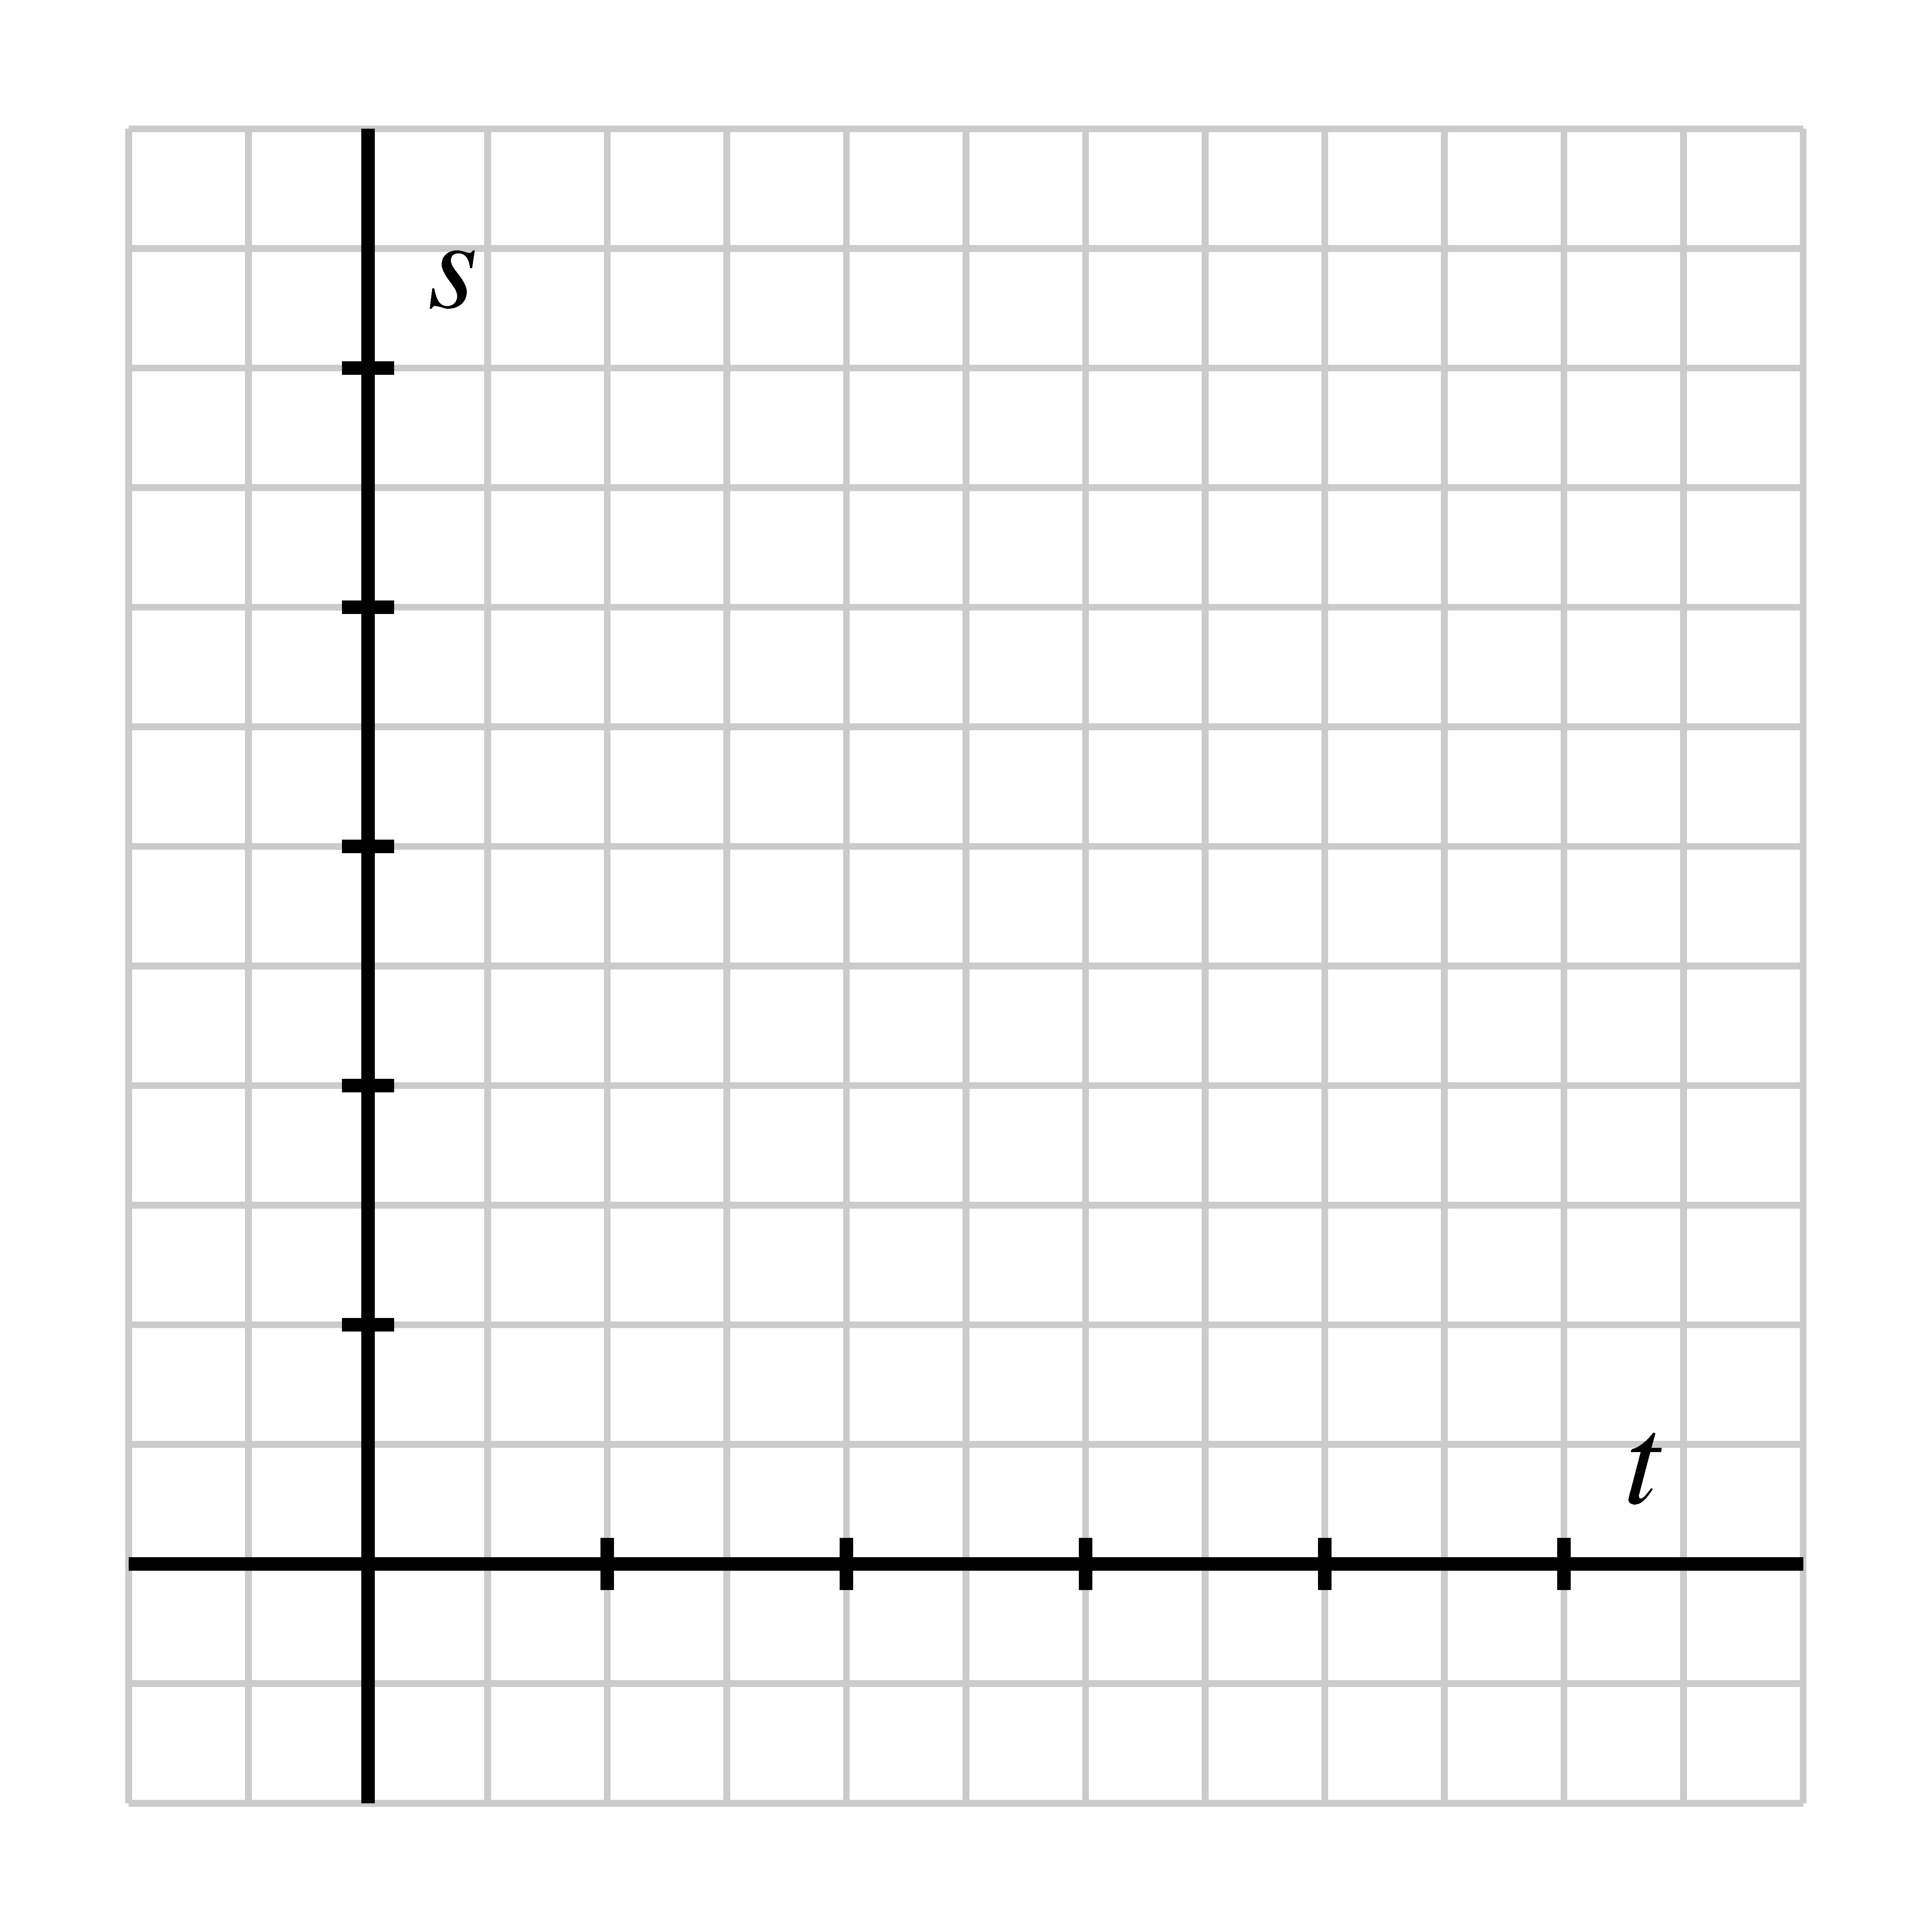
\includegraphics[width=.7\textwidth]{aroc-s-t-blank-axes.jpg}
\end{image}
\item Work by hand to find the equation of the line through the points $(1.5,s(1.5))$ and $(2.5, s(2.5))$. Write the line in the form $y = mt + b$ and plot the line in \emph{Desmos}, as well as on the axes above.
\item What is a geometric interpretation of the value $\av_{[1.5,2.5]}$ in light of your work in the preceding questions?
\item How do your answers in the preceding questions change if we instead consider the interval $[0.25, 0.75]$? $[0.5, 1.5]$? $[1,3]$?
\end{enumerate}
\end{exploration}


%\typeout{************************************************}
%\typeout{Defining and interpreting the average rate of change of a function}
%\typeout{************************************************}

\section{Defining and interpreting the average rate of change of a function}

In the context of a function that measures height or position of a moving object at a given time, the meaning of the average rate of change of the function on a given interval is the \emph{average velocity of the moving object} because it is the ratio of \emph{change in position} to \emph{change in time}.  For example, in the exploration above, the units on $\av_{[1.5,2.5]} = -32$ are ``feet per second'' since the units on the numerator are ``feet'' and on the denominator ``seconds''.  Morever, $-32$ is numerically the same value as the slope of the line that connects the two corresponding points on the graph of the position function, as seen below.  The fact that the average rate of change is negative in this example indicates that the ball is falling.

\begin{image}
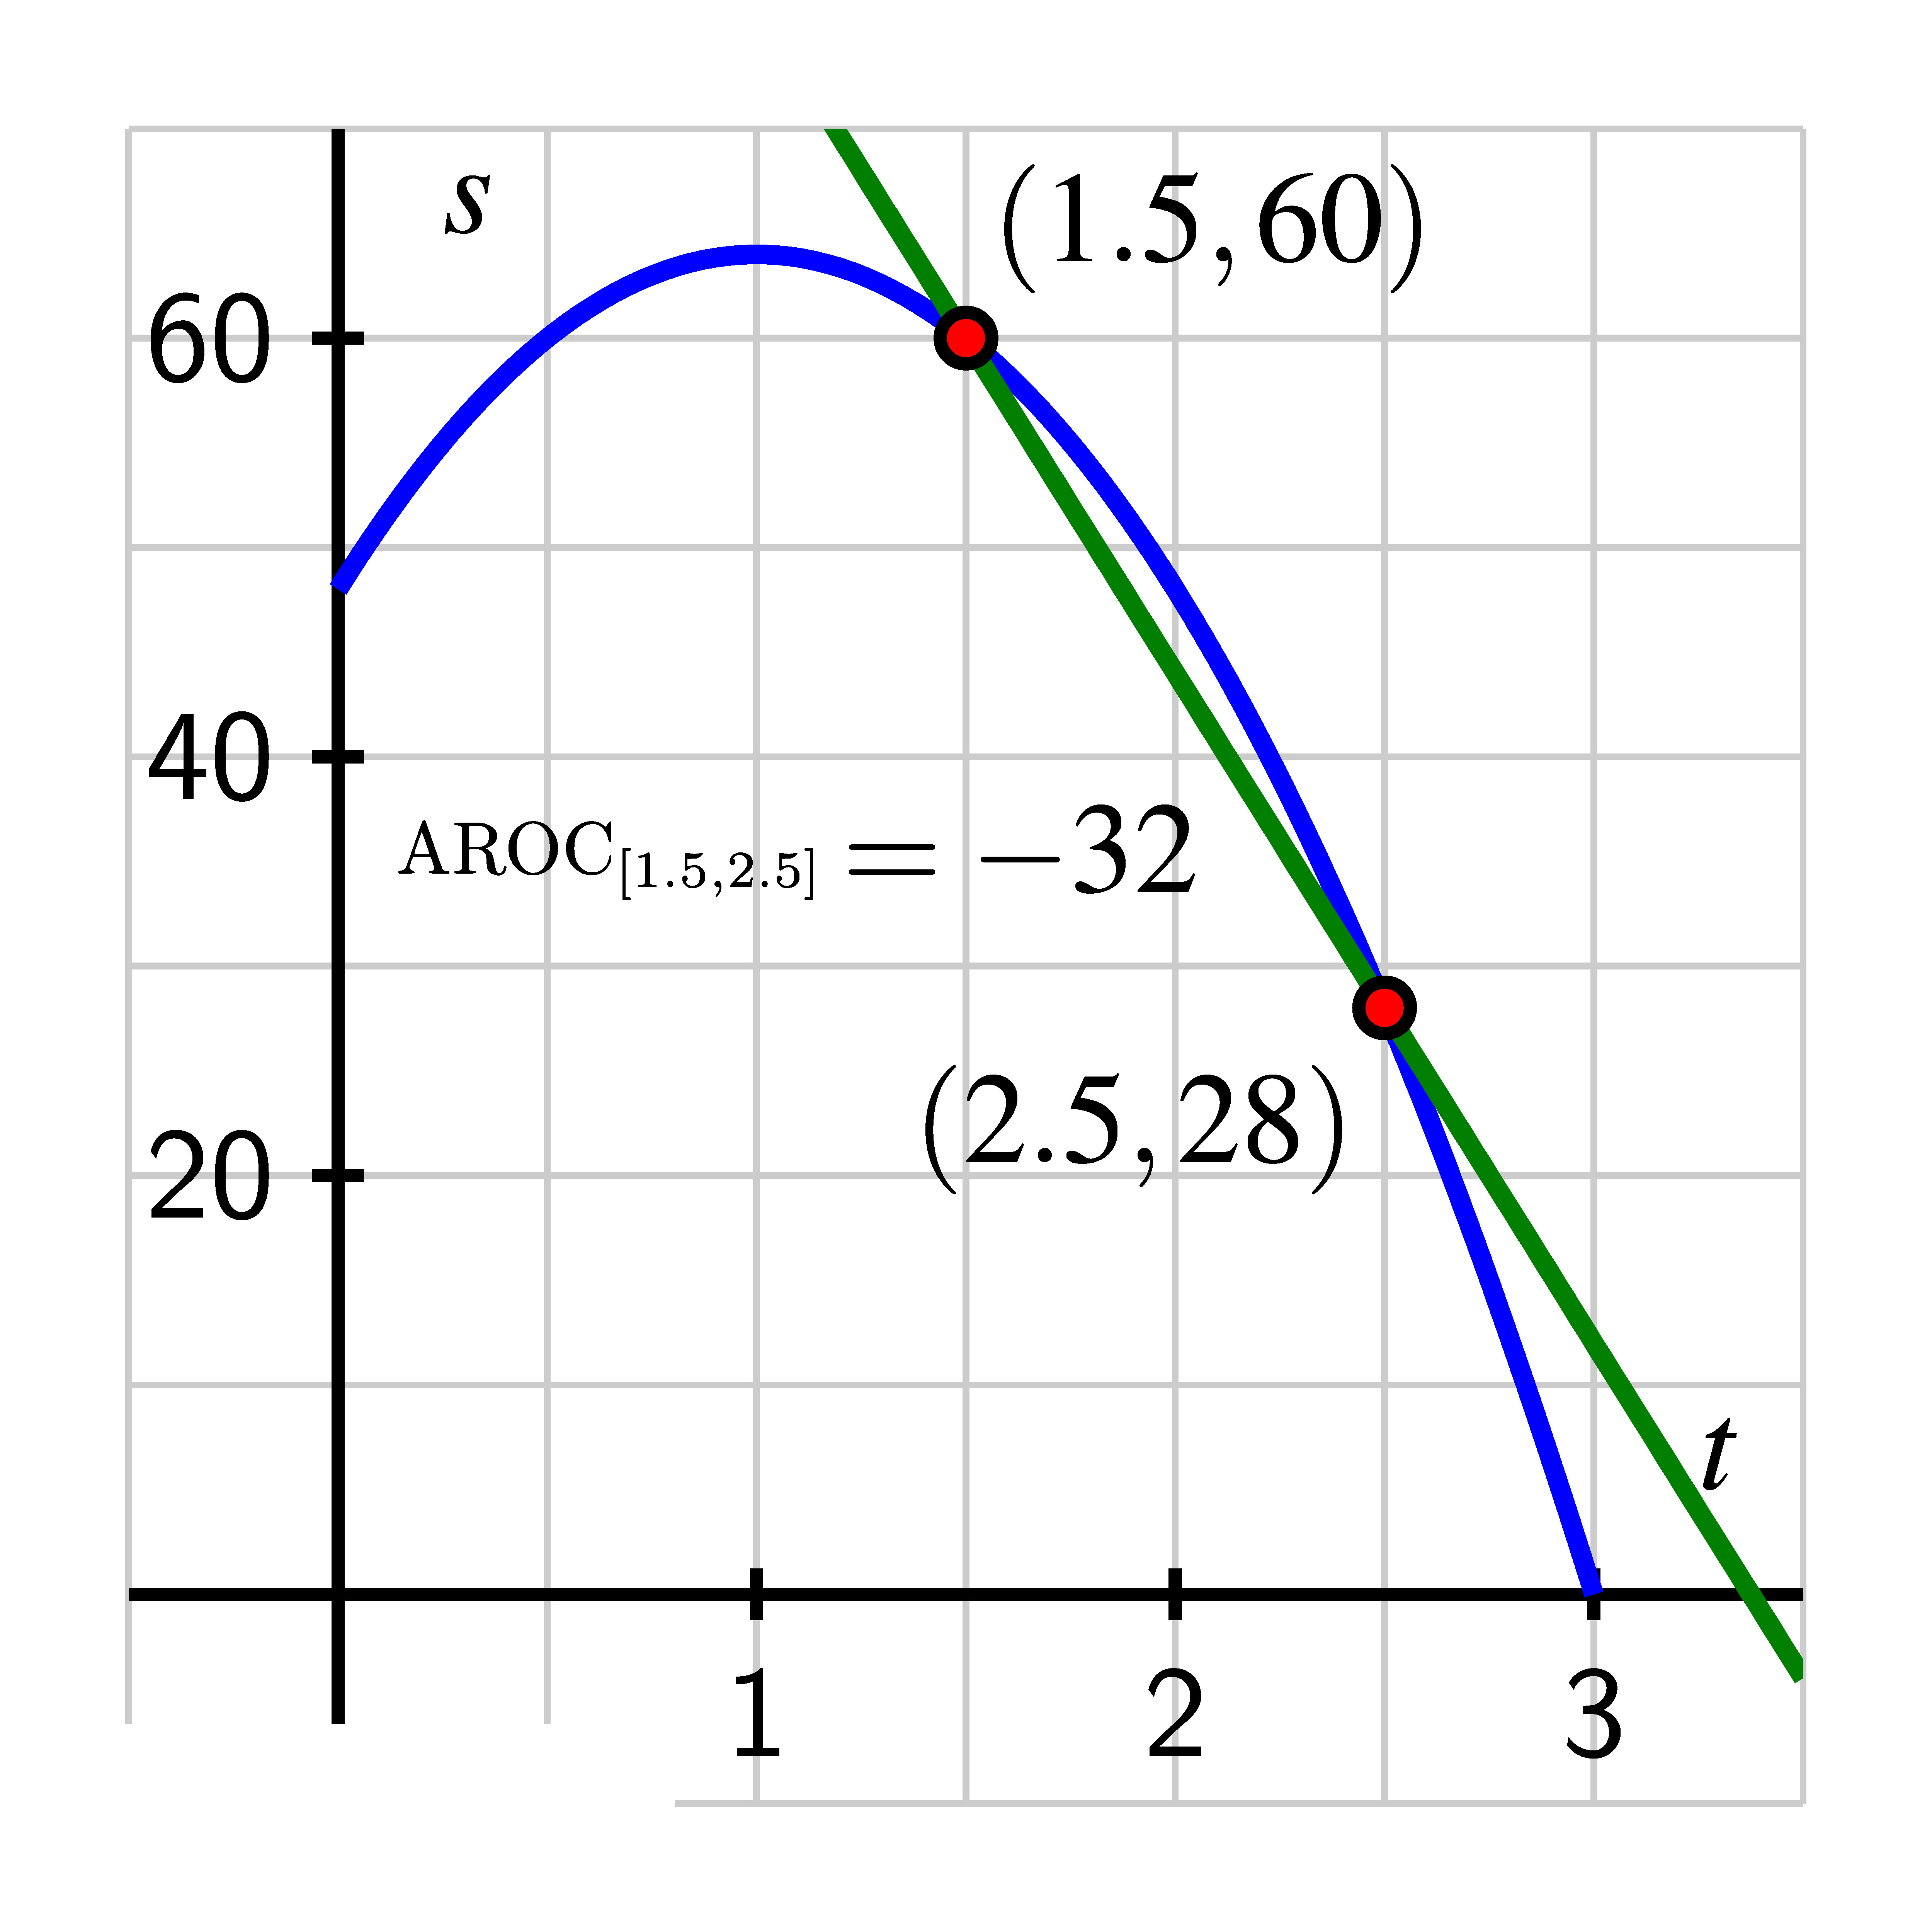
\includegraphics[width=.7\textwidth]{aroc-s-t-ex-1.jpg}
\end{image}

While the average rate of change of a position function tells us the moving object's average velocity, in other contexts, the average rate of change of a function can be similarly defined and has a related interpretation.  We make the following formal definition.

\begin{definition}
For a function $f$ defined on an interval $[a,b]$, the \dfn{average rate of change of $f$ between $(a,f(a))$ and $(b,f(b))$} is the quantity%
\begin{equation*}
\av_{[a,b]} = \frac{f(b) - f(a)}{b-a}\text{.}
\end{equation*}

\begin{image}
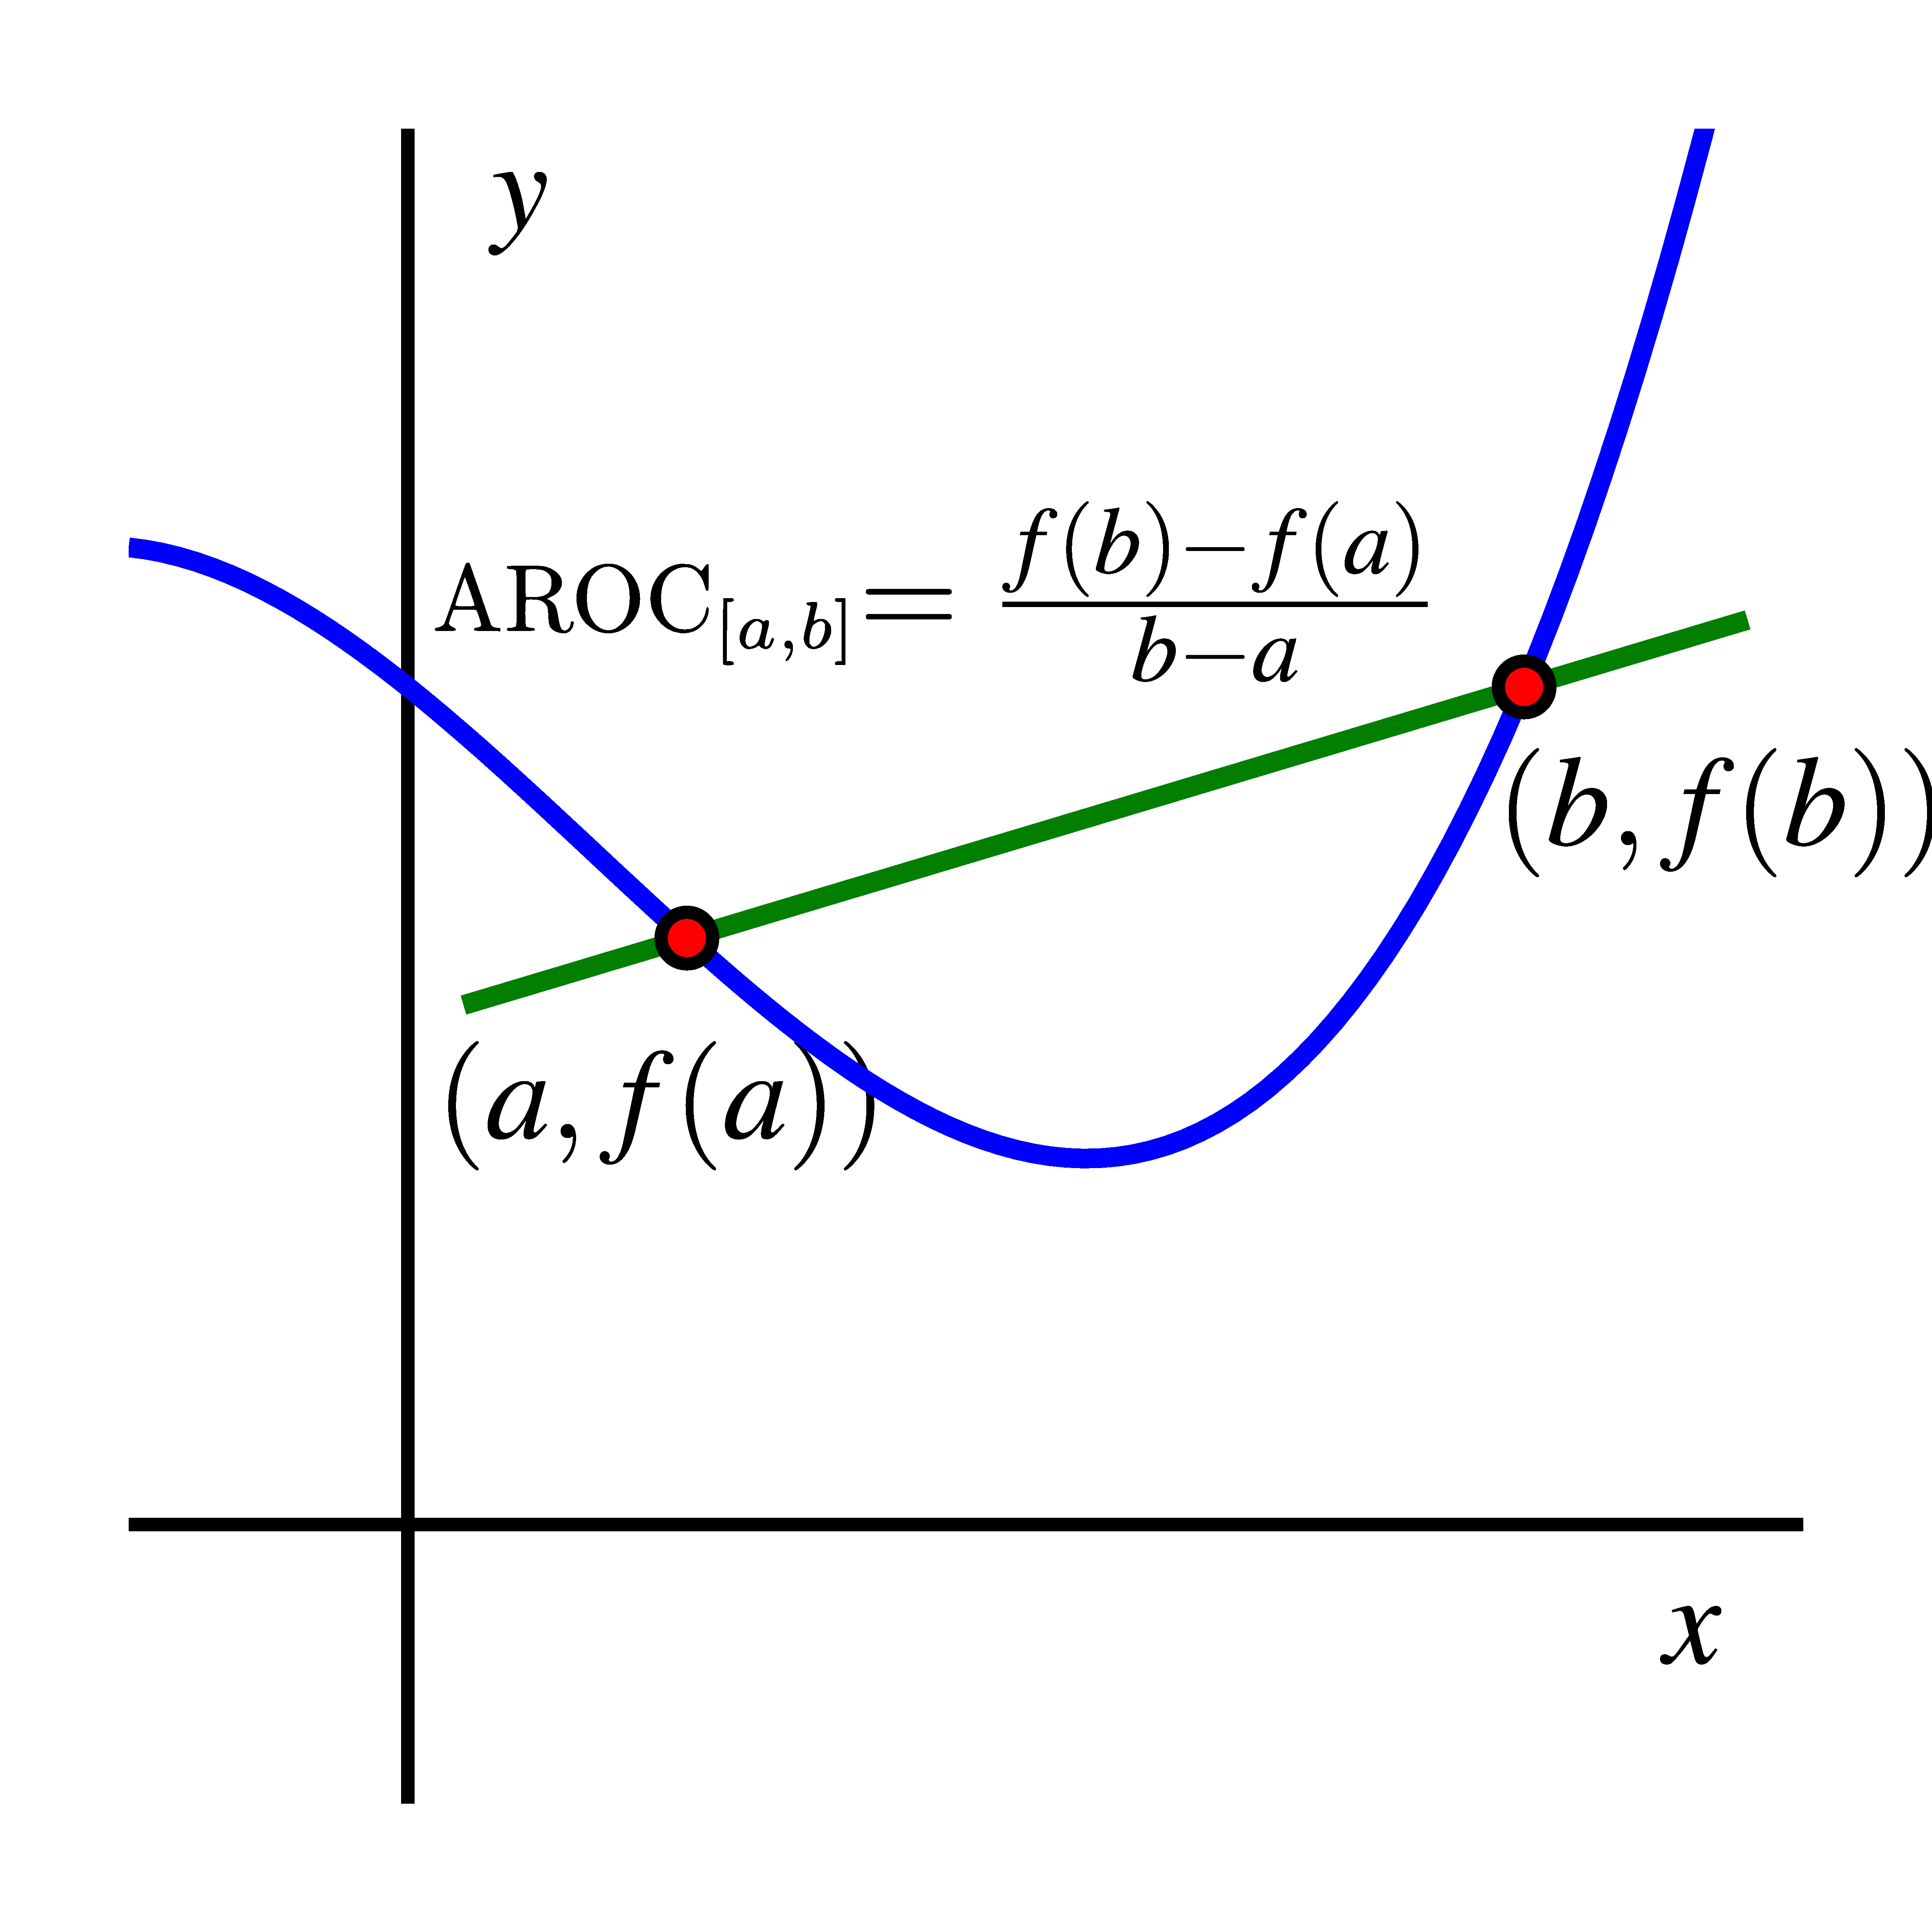
\includegraphics[width=.7\textwidth]{aroc-f-x-defn.jpg}
\end{image}

\end{definition}
In every situation, the units on the average rate of change help us interpret its meaning, and those units are always ``units of output per unit of input.'' \index{average rate of change!units}  Moreover, the average rate of change of $f$ on $[a,b]$ always corresponds to the slope of the line between the points $(a,f(a))$ and $(b,f(b))$. Before we explore this concept further, we note that this line has a special name, it is the \textit{secant line} to the graph. 

\begin{callout}
  {\bf Definition:} Consider a function $y=f(x)$. A line passing through two points $(a,f(a))$ and $(b,f(b))$, with $a \neq b$, in the graph of $y=f(x)$, is called a \textbf{secant line} to the graph. The slope of a secant line is the average rate of change of the function on the interval $[a,b]$.
\end{callout}

\begin{exploration}
According to the US census, the populations of Kent and Ottawa Counties (Grand Rapids is in Kent, Allendale in Ottawa) from 1960 to 2010 measured in $10$-year intervals are given in the following tables.

\begin{center}

\textbf{Kent County Population data}
$
\begin{array}{llllll}
1960&1970&1980&1990&2000&2010\\
\hline
363,187&411,044&444,506&500,631&574,336&602,622
\end{array}
$

\vspace{.2in}

\textbf{Ottawa County Population data}
$
\begin{array}{llllll}
1960&1970&1980&1990&2000&2010\\
\hline
98,719&128,181&157,174&187,768&238,313&263,801
\end{array}
$
\end{center}

Let $K(Y)$ represent the population of Kent County in year $Y$ and $W(Y)$ the population of Ottawa County in year Y.
\begin{enumerate}[label=\alph*.]
\item Compute $\av_{[1990,2010]}$ for both $K$ and $O$.
\item What are the units on each of the quantities you computed in (a.)?
\item Write a careful sentence that explains the meaning of the average rate of change of the Ottawa county population on the time interval $[1990,2010]$.  Your sentence should begin something like ``In an average year between 1990 and 2010, the population of Ottawa County was $\ldots$''
\item Which county had a greater average rate of change during the time interval $[2000,2010]$? Were there any intervals in which one of the counties had a negative average rate of change?
\item Using the given data, what do you predict will be the population of Ottawa County in 2018? Why?
\end{enumerate}
\end{exploration}

The average rate of change of a function on an interval gives us an excellent way to describe how the function behaves, on average.  For instance, if we compute $\av_{[1970,2000]}$ for Kent County, we find that%
\begin{equation*}
\av_{[1970,2000]} = \frac{573,336 - 411,044}{30} \approx 5409.73\text{,} \calcHW
\end{equation*}
which tells us that in an average year from 1970 to 2000, the population of Kent County increased by about $5410$ people.  Said differently, we could also say that from 1970 to 2000, Kent County was growing at an average rate of $5410$ people per year.  These ideas also afford the opportunity to make comparisons over time.  Since%
\begin{equation*}
\av_{[1990,2000]} = \frac{573,336 - 500,631}{30} = 7270.5\text{,} \calcHW
\end{equation*}
we can not only say that the county's population increased by about $7270$ in an average year between 1990 and 2000, but also that the population was growing faster from 1990 to 2000 than it did from 1970 to 2000.%

Finally, we can even use the average rate of change of a function to predict future behavior.  Since the population was changing on average by $7270.5$ people per year from 1990 to 2000, we can estimate that the population in 2002 is%
\begin{equation*}
K(2002) \approx K(2000) + 2 \cdot 7270.5 = 573,336 + 14,541 = 587,877\text{.}
\end{equation*}


%\typeout{************************************************}
%\typeout{How average rate of change indicates function trends}
%\typeout{************************************************}

\section{How average rate of change indicates function trends}

We have already seen that it is natural to use words such as ``increasing'' and ``decreasing'' to describe a function's behavior.  For instance, for the tennis ball whose height is modeled by $s(t) = 64 - 16(t-1)^2$, we computed that $\av_{[1.5,2.5]} = -32$, which indicates that on the interval $[1.5,2.5]$, the tennis ball's height is decreasing at an average rate of $32$ feet per second.  Similarly, for the population of Kent County, since $\av_{[1990,2000]} = 7270.5$, we know that on the interval $[1990,2000]$ the population is increasing at an average rate of $7270.5$ people per year.

We make the following formal definitions to clarify what it means to say that a function is increasing or decreasing.

\begin{definition}
Let $f$ be a function defined on an interval $(a,b)$ (that is, on the set of all $x$ for which $a < x < b$).  We say that $f$ is \dfn{increasing on $(a,b)$} provided that the function is always rising as we move from left to right.  That is, for any $x$ and $y$ in $(a,b)$, if $x < y$, then $f(x) < f(y)$.%
\\
\\
Similarly, we say that $f$ is \dfn{decreasing on $(a,b)$} provided that the function is always falling as we move from left to right.  That is, for any $x$ and $y$ in $(a,b)$,  if $x < y$, then $f(x) > f(y)$.%
\end{definition}

If a function is increasing, its average rate of change will be positive. If a function is decreasing, its average rate of change will be negative. However the reverse doesn't necessarily hold true.
If we compute the average rate of change of a function on an interval, we can decide if the function is increasing or decreasing \emph{on average} on the interval, but it takes more work\footnote{Calculus offers one way to justify that a function is always increasing or always decreasing on an interval.\label{fn-7}} to decide if the function is increasing or decreasing \emph{always} on the interval.

\begin{exploration}
Let's consider two different functions and see how different computations of their average rate of change tells us about their respective behavior. Plots of $q$  and $h$ are shown below.

\begin{enumerate}[label=\alph*.]
\item Consider the function $q(x) = 4-(x-2)^2$. Compute $\av_{[0,1]}$, $\av_{[1,2]}$, $\av_{[2,3]}$, and $\av_{[3,4]}$. What do your last two computations tell you about the behavior of the function $q$ on $[2,4]$?


\item Consider the function $h(t) = 3 - 2(0.95)^t$. Compute $\av_{[-1,1]}$, $\av_{[1,3]}$, and $\av_{[3,5]}$. What do your computations tell you about the behavior of the function $h$ on $[-1,5]$?

\item On the graphs below, plot the line segments whose respective slopes are the average rates of change you computed in (a) and (b).

\begin{image}
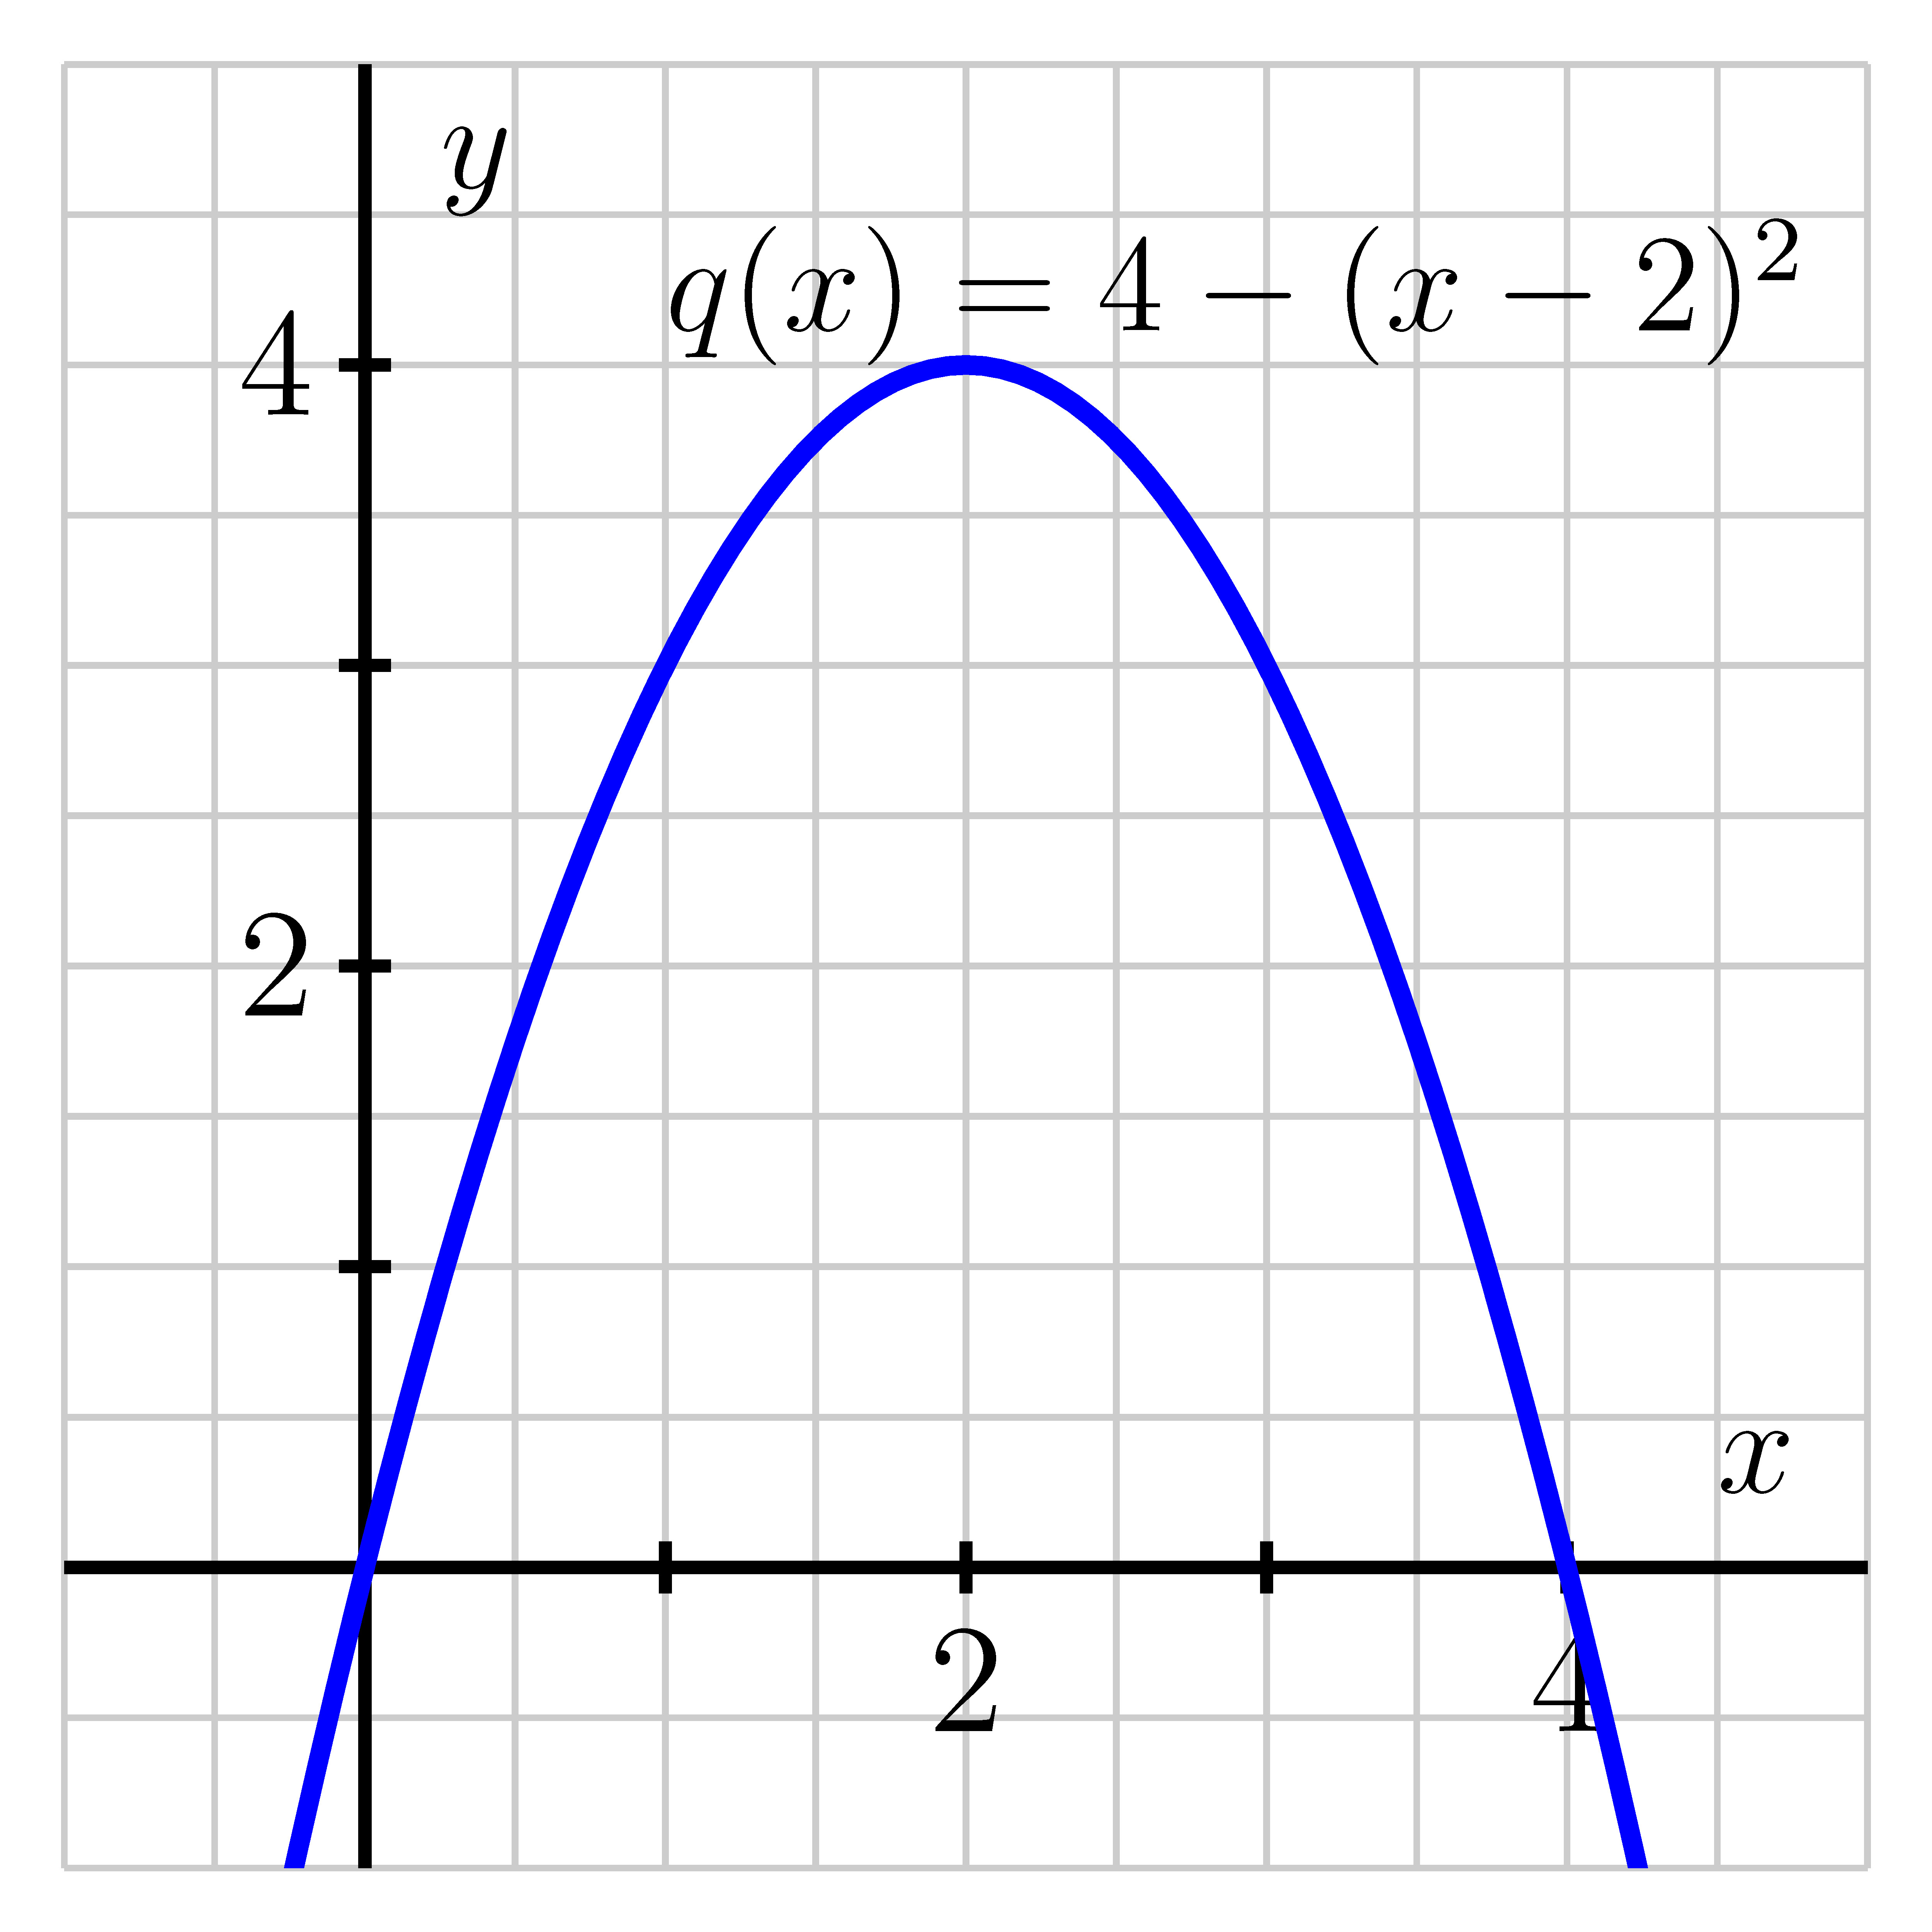
\includegraphics[width=.7\textwidth]{aroc-act-trends-q.jpg}
\end{image}

\begin{image}
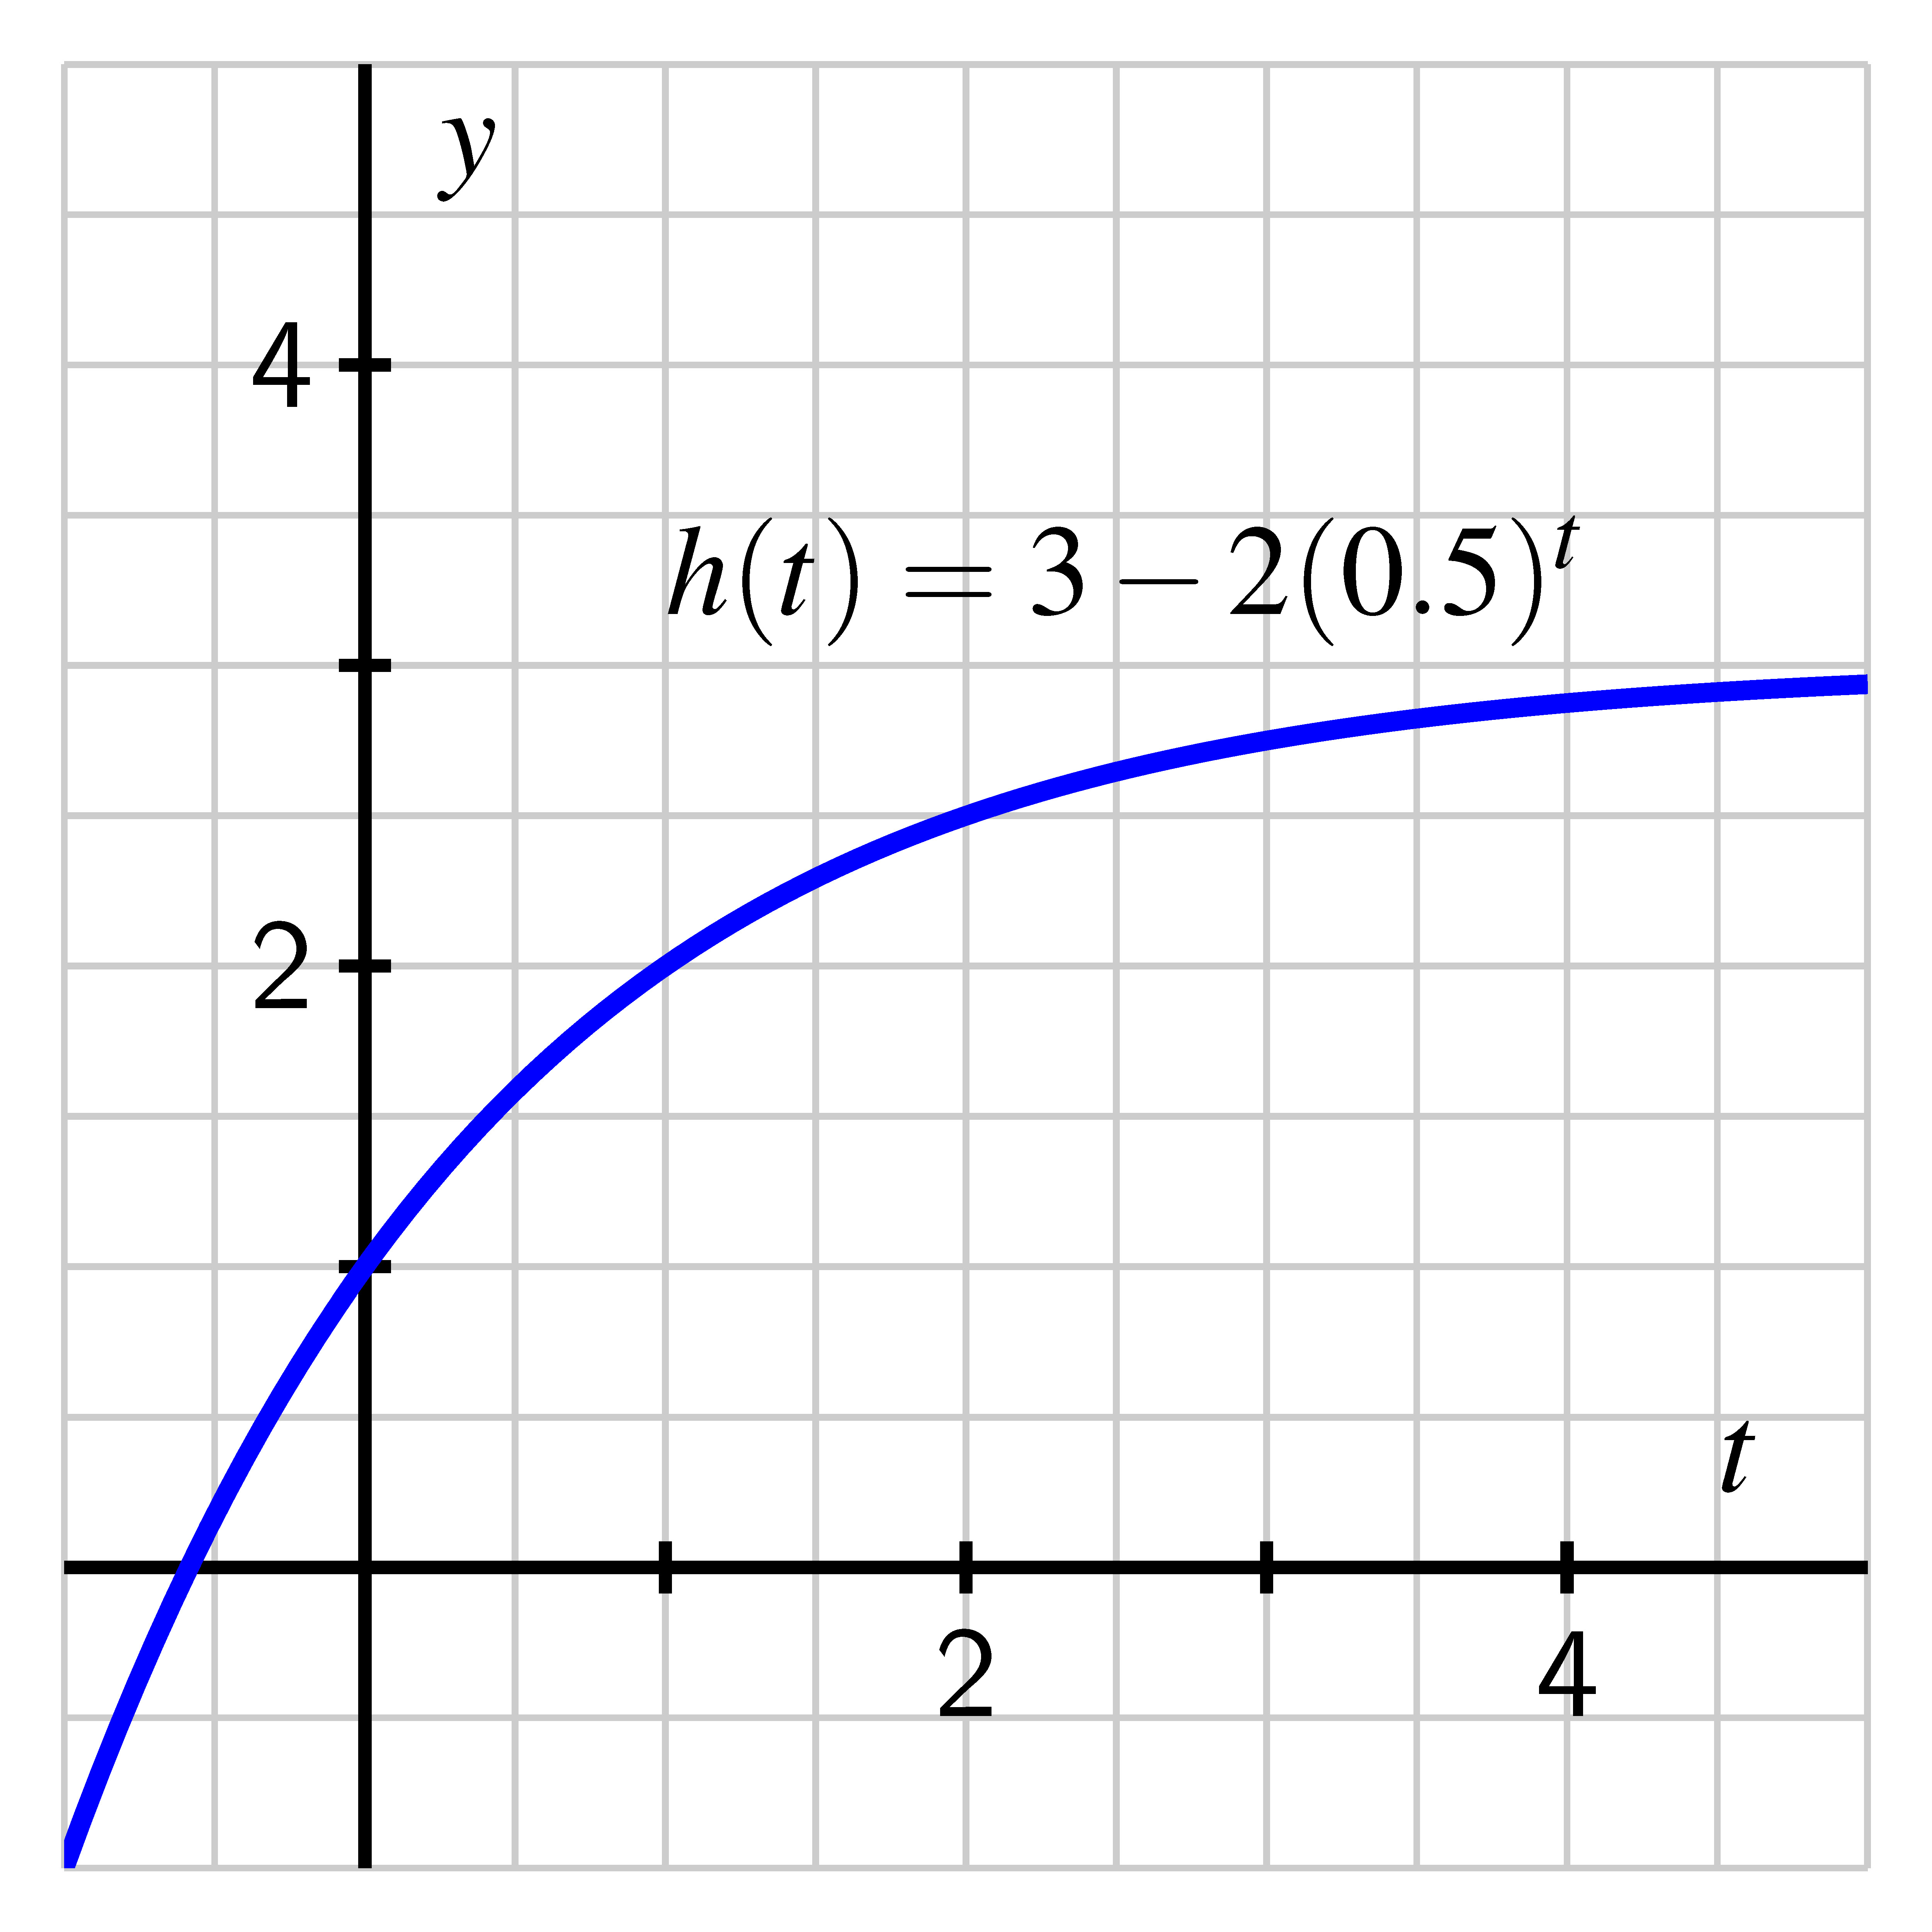
\includegraphics[width=.7\textwidth]{aroc-act-trends-h.jpg}
\end{image}

\item True or false: Since $\av_{[0,3]} = 1$, the function $q$ is increasing on the interval $(0,3)$.  Justify your decision.
\item Give an example of a function that has the same average rate of change no matter what interval you choose. You can provide your example through a table, a graph, or a formula; regardless of your choice, write a sentence to explain.
\end{enumerate}

\end{exploration}

It is helpful be able to connect information about a function's average rate of change and its graph.  For instance, if we have determined that $\av_{[-3,2]} = 1.75$ for some function $f$, this tells us that, on average, the function rises between the points $x = -3$ and $x = 2$ and does so at an average rate of $1.75$ vertical units for every horizontal unit.  Moreover, we can even determine that the difference between $f(2)$ and $f(-3)$ is%
\begin{equation*}
f(2)-f(-3) = 1.75 \cdot 5 = 8.75
\end{equation*}
since $\frac{f(2)-f(-3)}{2-(-3)} = 1.75$.

\begin{exploration}
Sketch at least two different possible graphs that satisfy the criteria for the function stated in each part.  Make your graphs as significantly different as you can.  If it is impossible for a graph to satisfy the criteria, explain why.



\begin{enumerate}[label=\alph*.]
\item 
$f$ is a function defined on $[-1,7]$ such that $f(1) = 4$ and $\av_{[1,3]} = -2$.

	\begin{center}
	$
	\begin{array}{ccc}
	{
	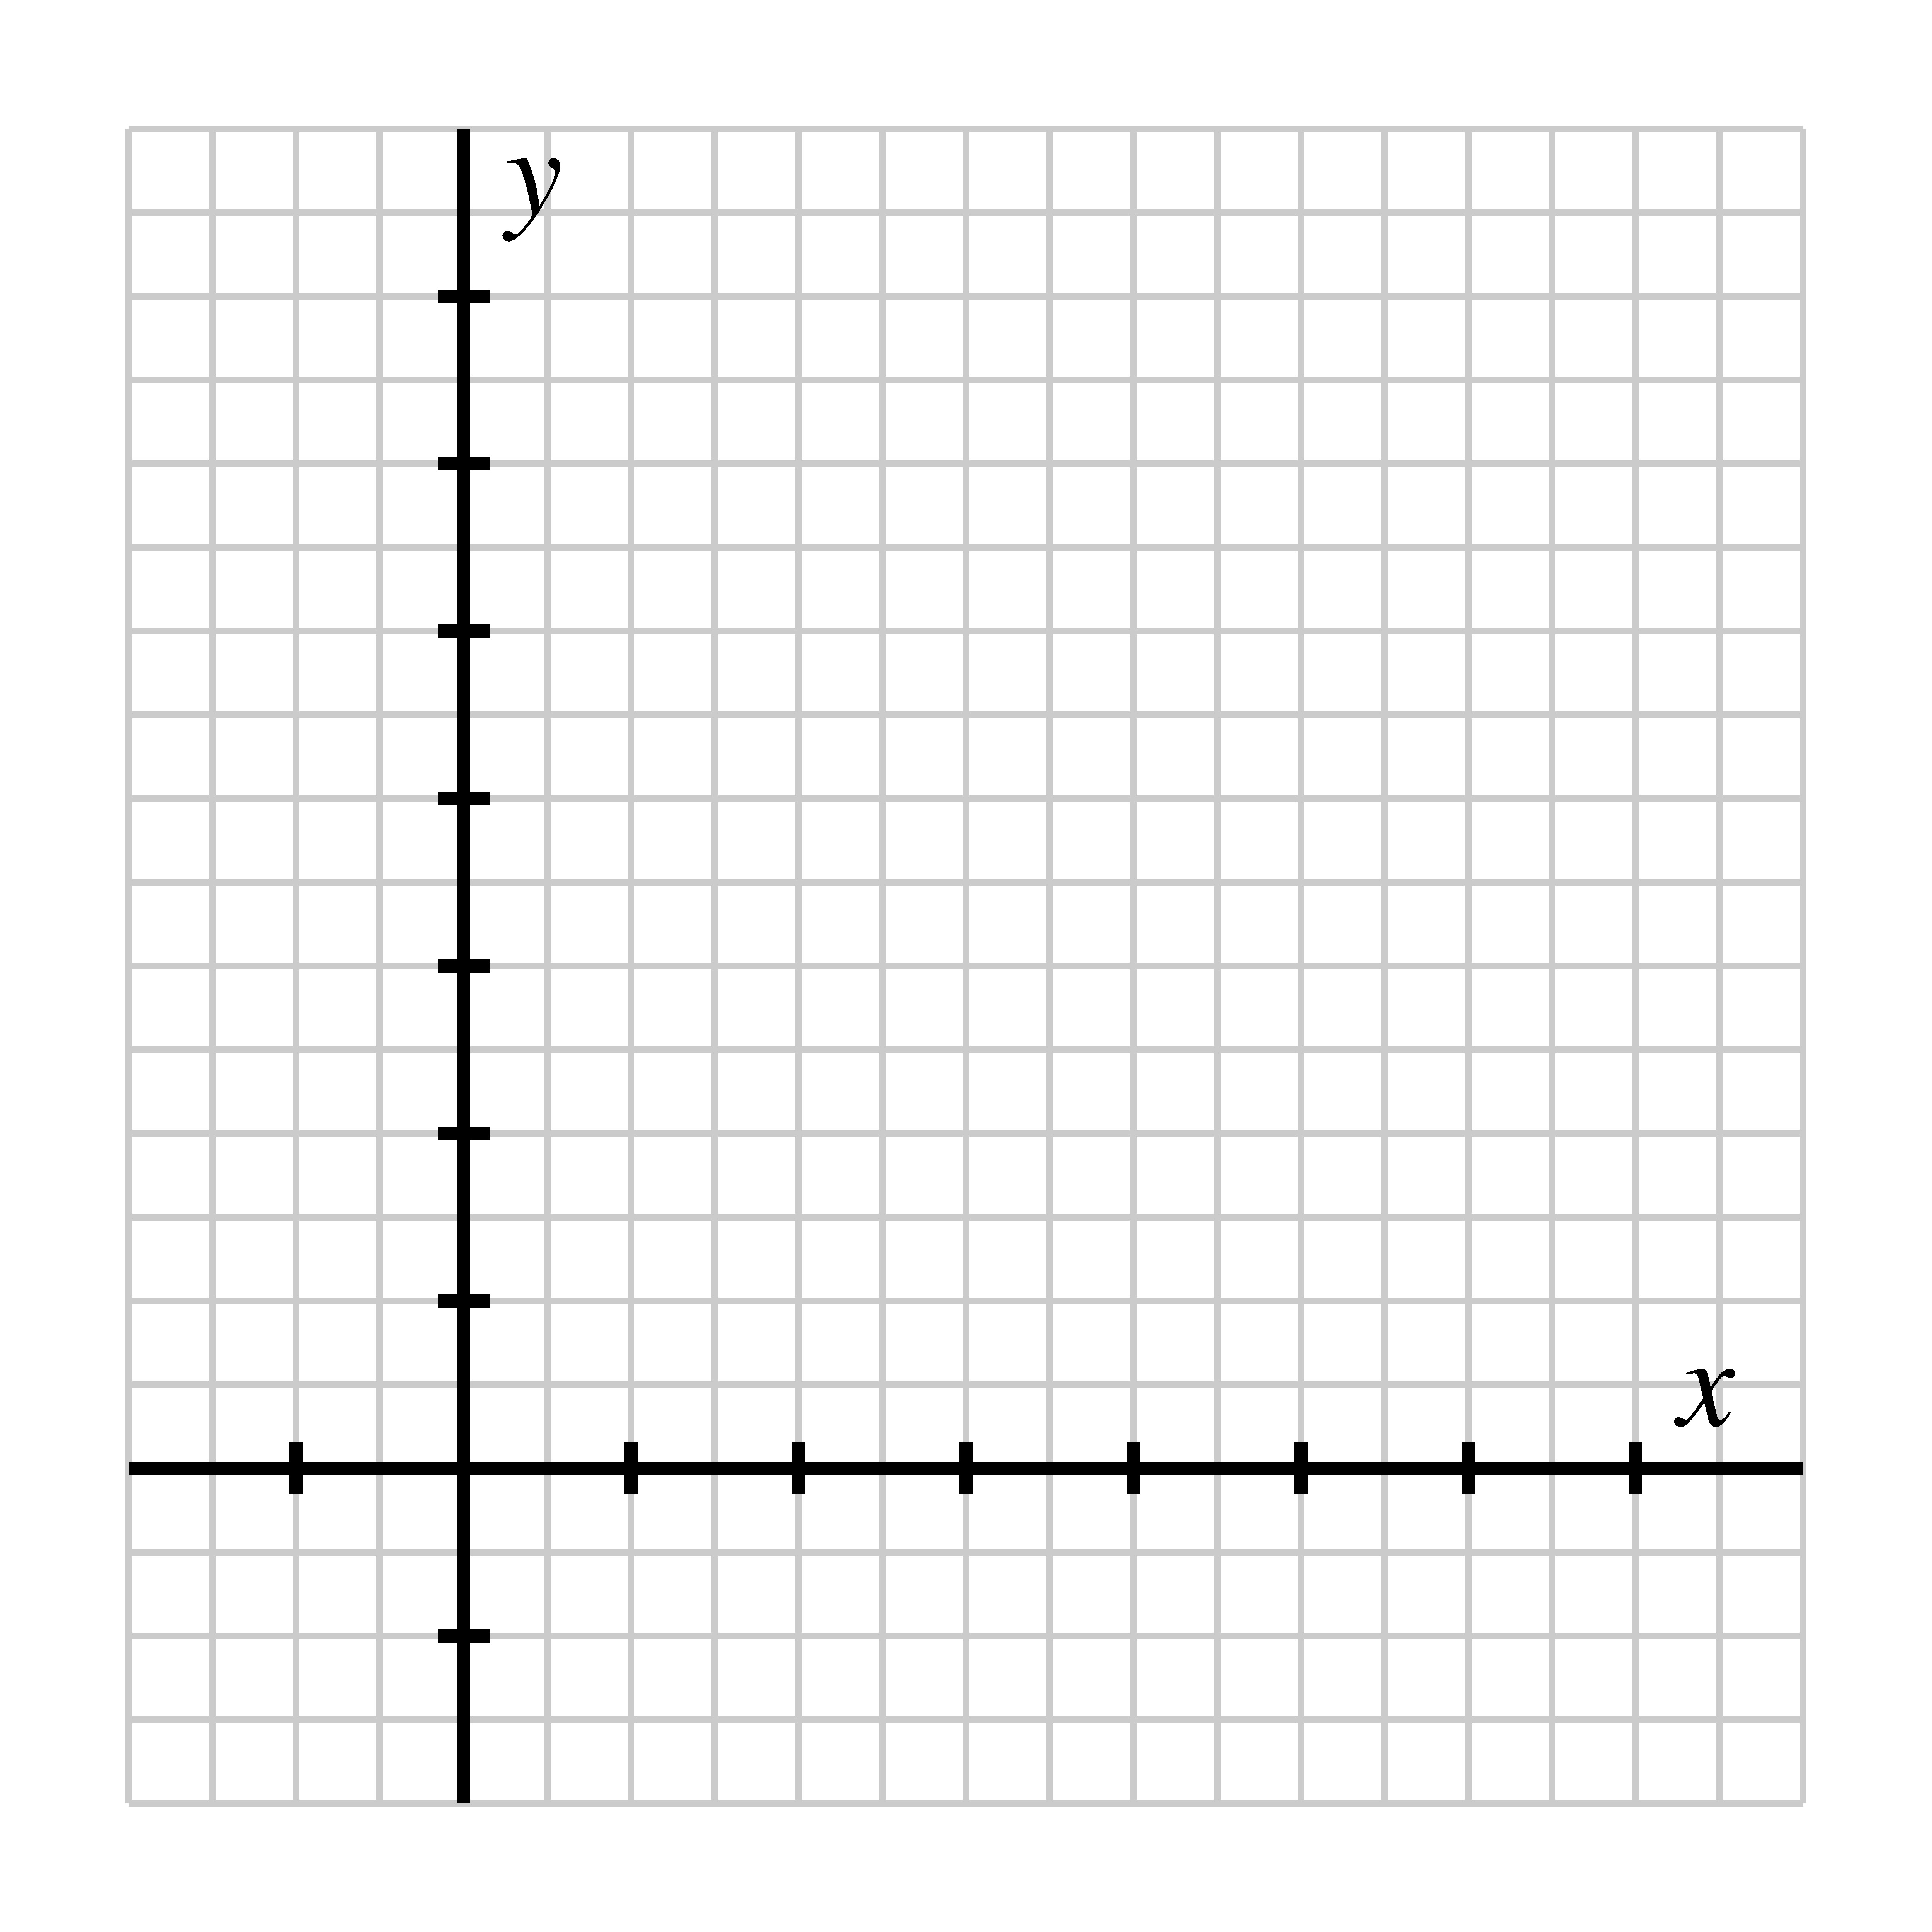
\includegraphics[width=.4\textwidth]{functions-y-x-blank-axes.jpg}
	}&&
	{
	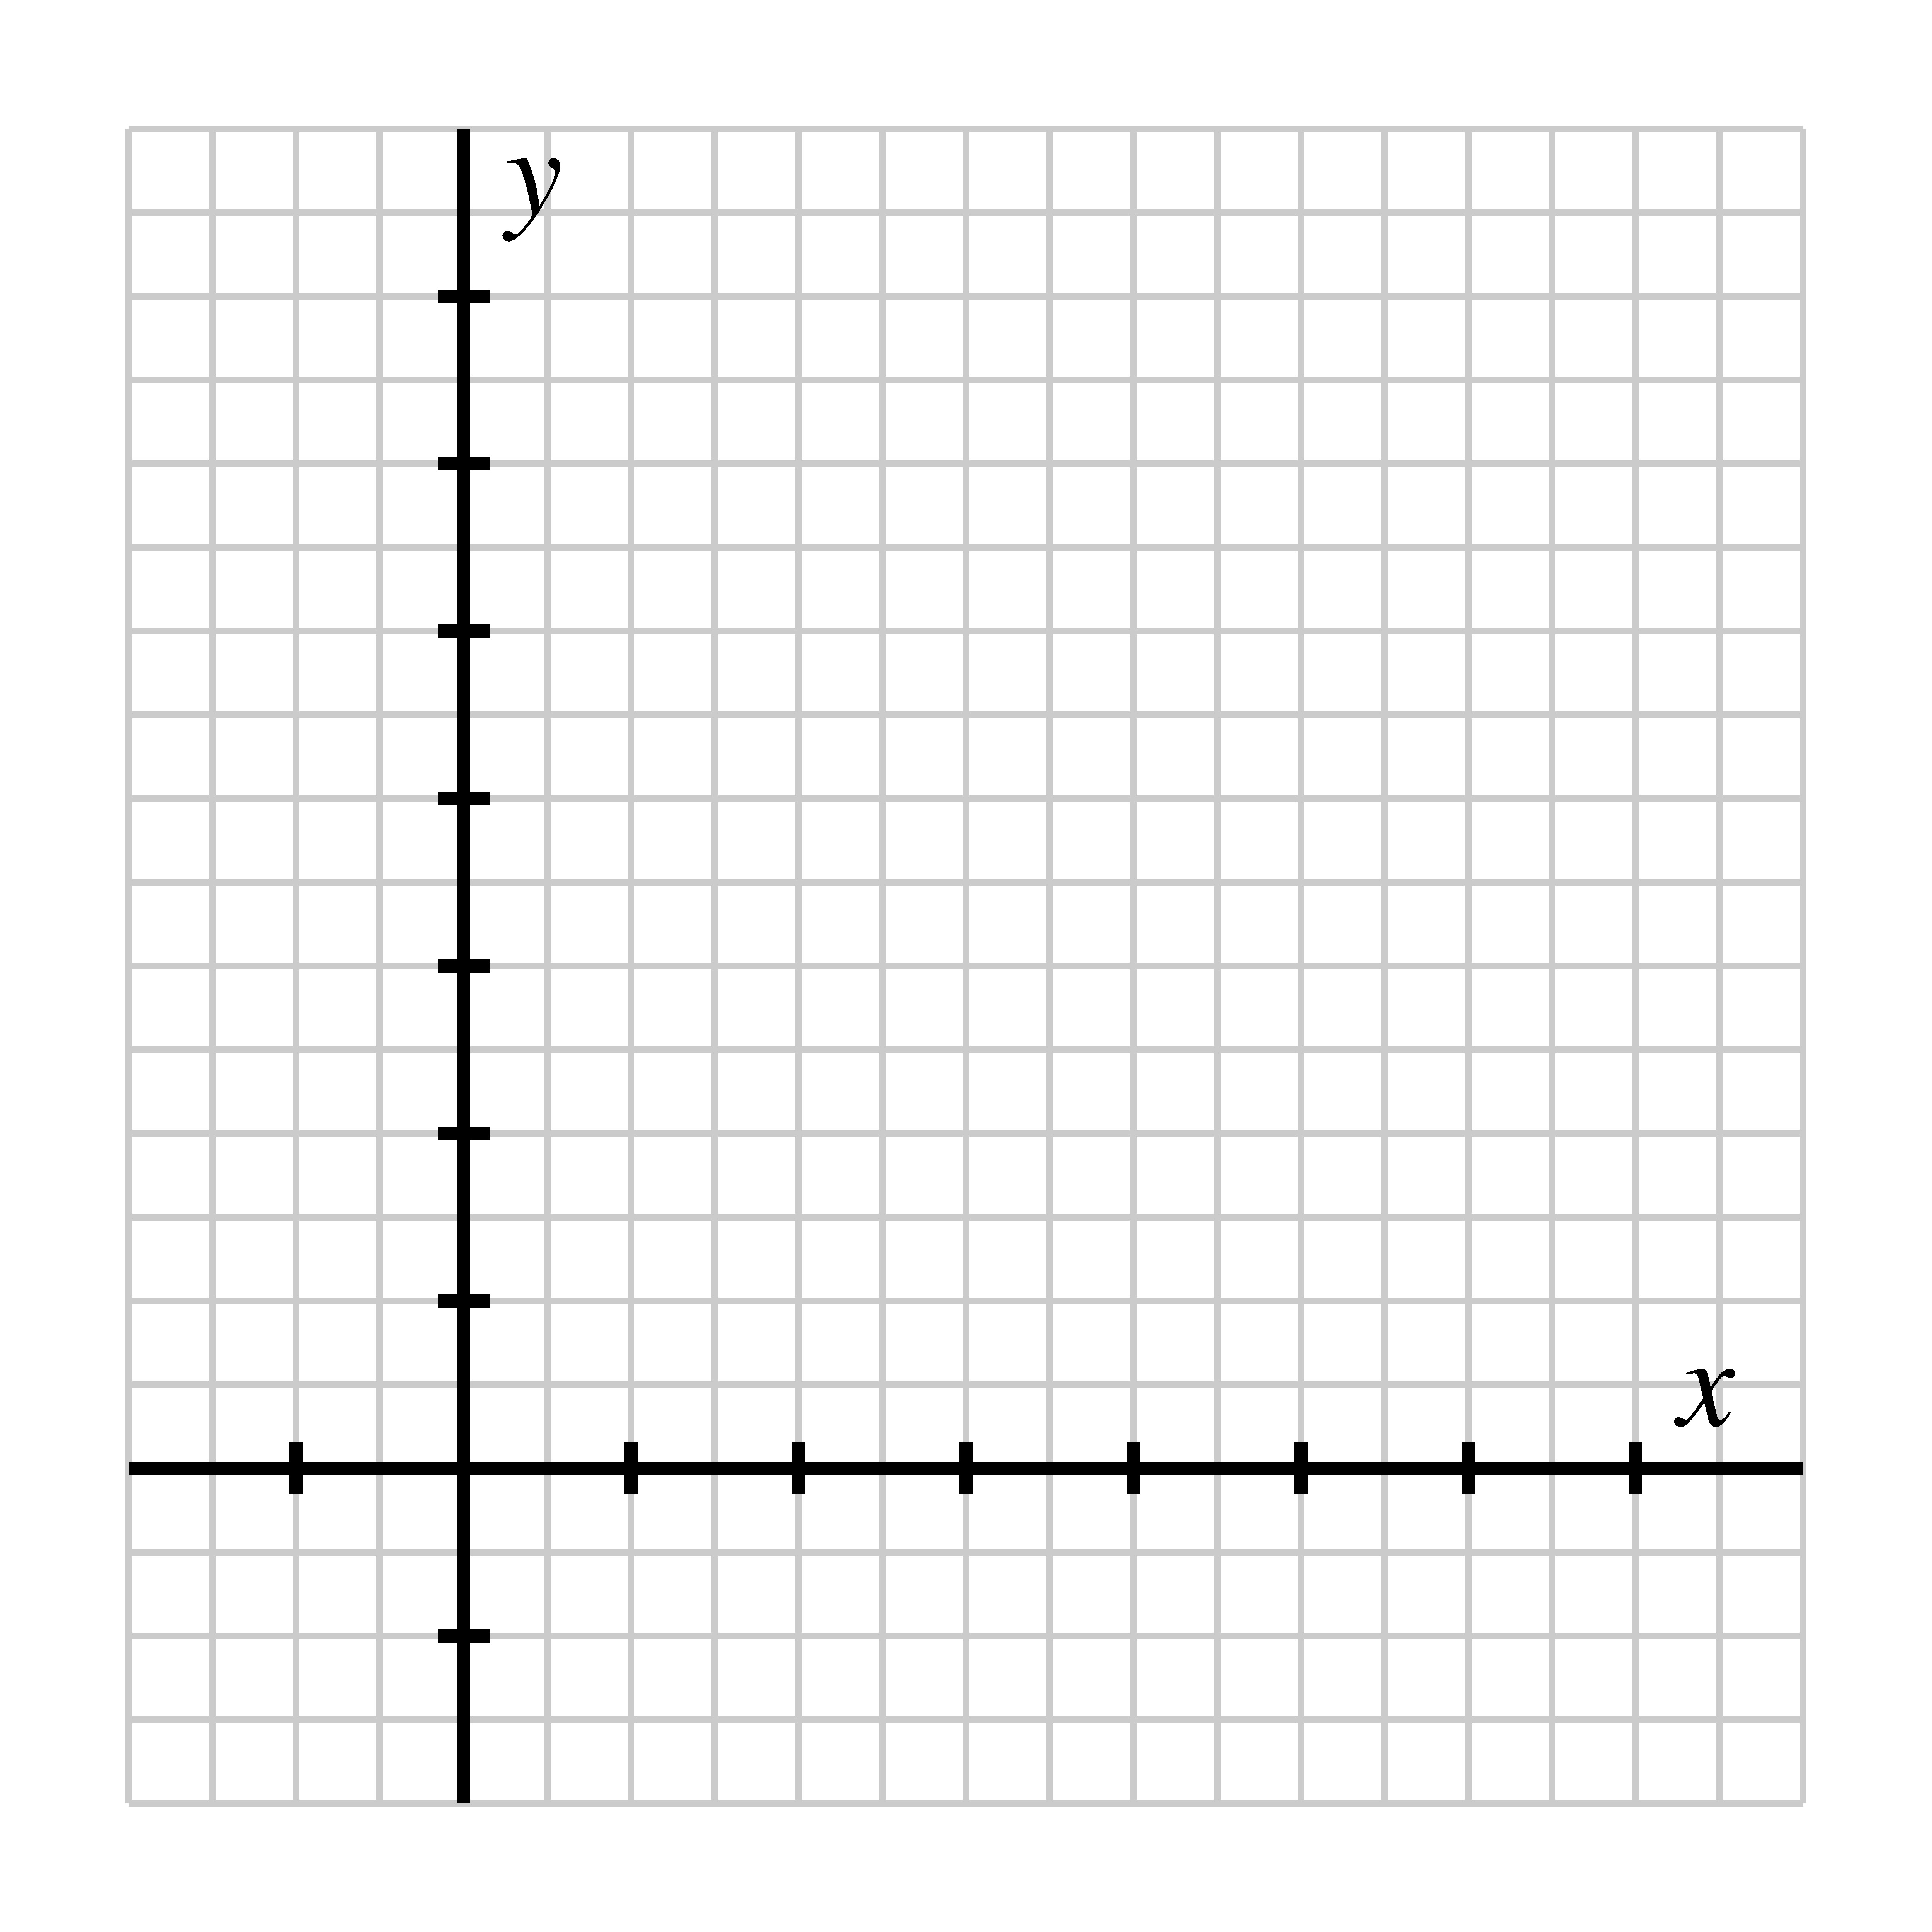
\includegraphics[width=.4\textwidth]{functions-y-x-blank-axes.jpg}
	}\\
	\end{array}
	$
	\end{center}

\item $g$ is a function defined on $[-1,7]$ such that $g(4) = 3$, $\av_{[0,4]}=\frac{1}{2}$, and $g$ is not always increasing on $(0,4)$.

	\begin{center}
	$
	\begin{array}{ccc}
	{
	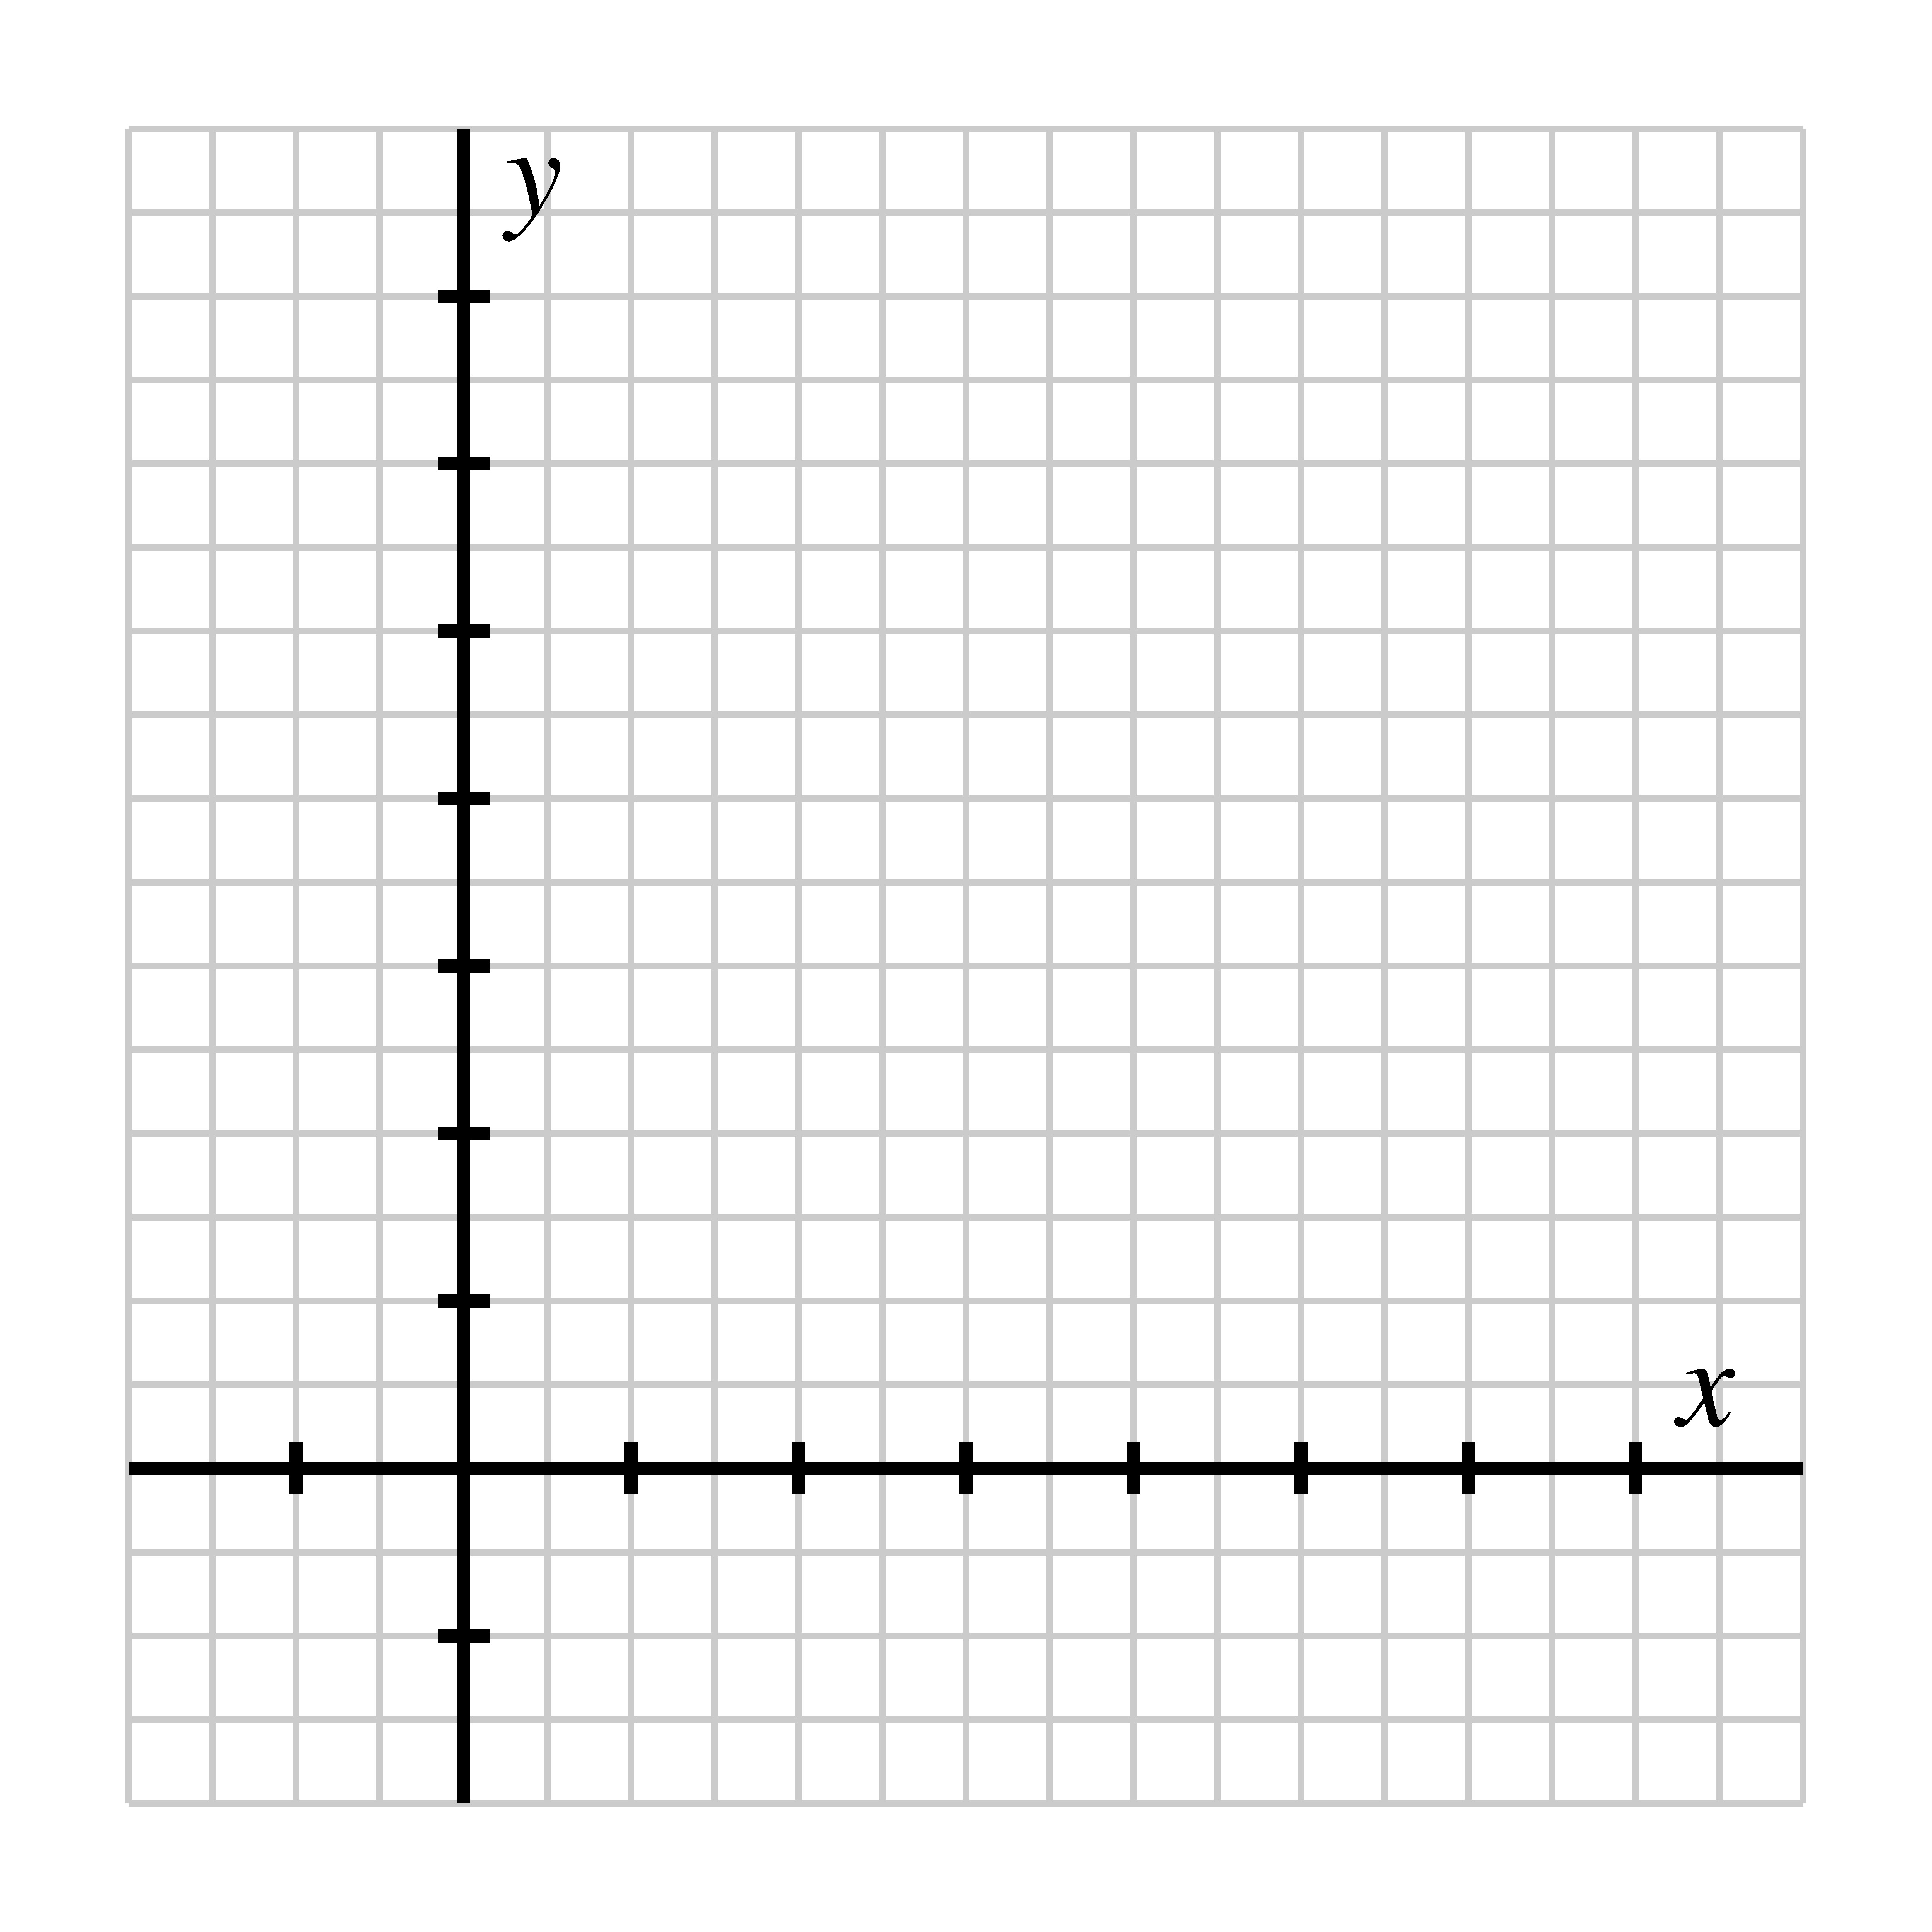
\includegraphics[width=.4\textwidth]{functions-y-x-blank-axes.jpg}
	}&&
	{
	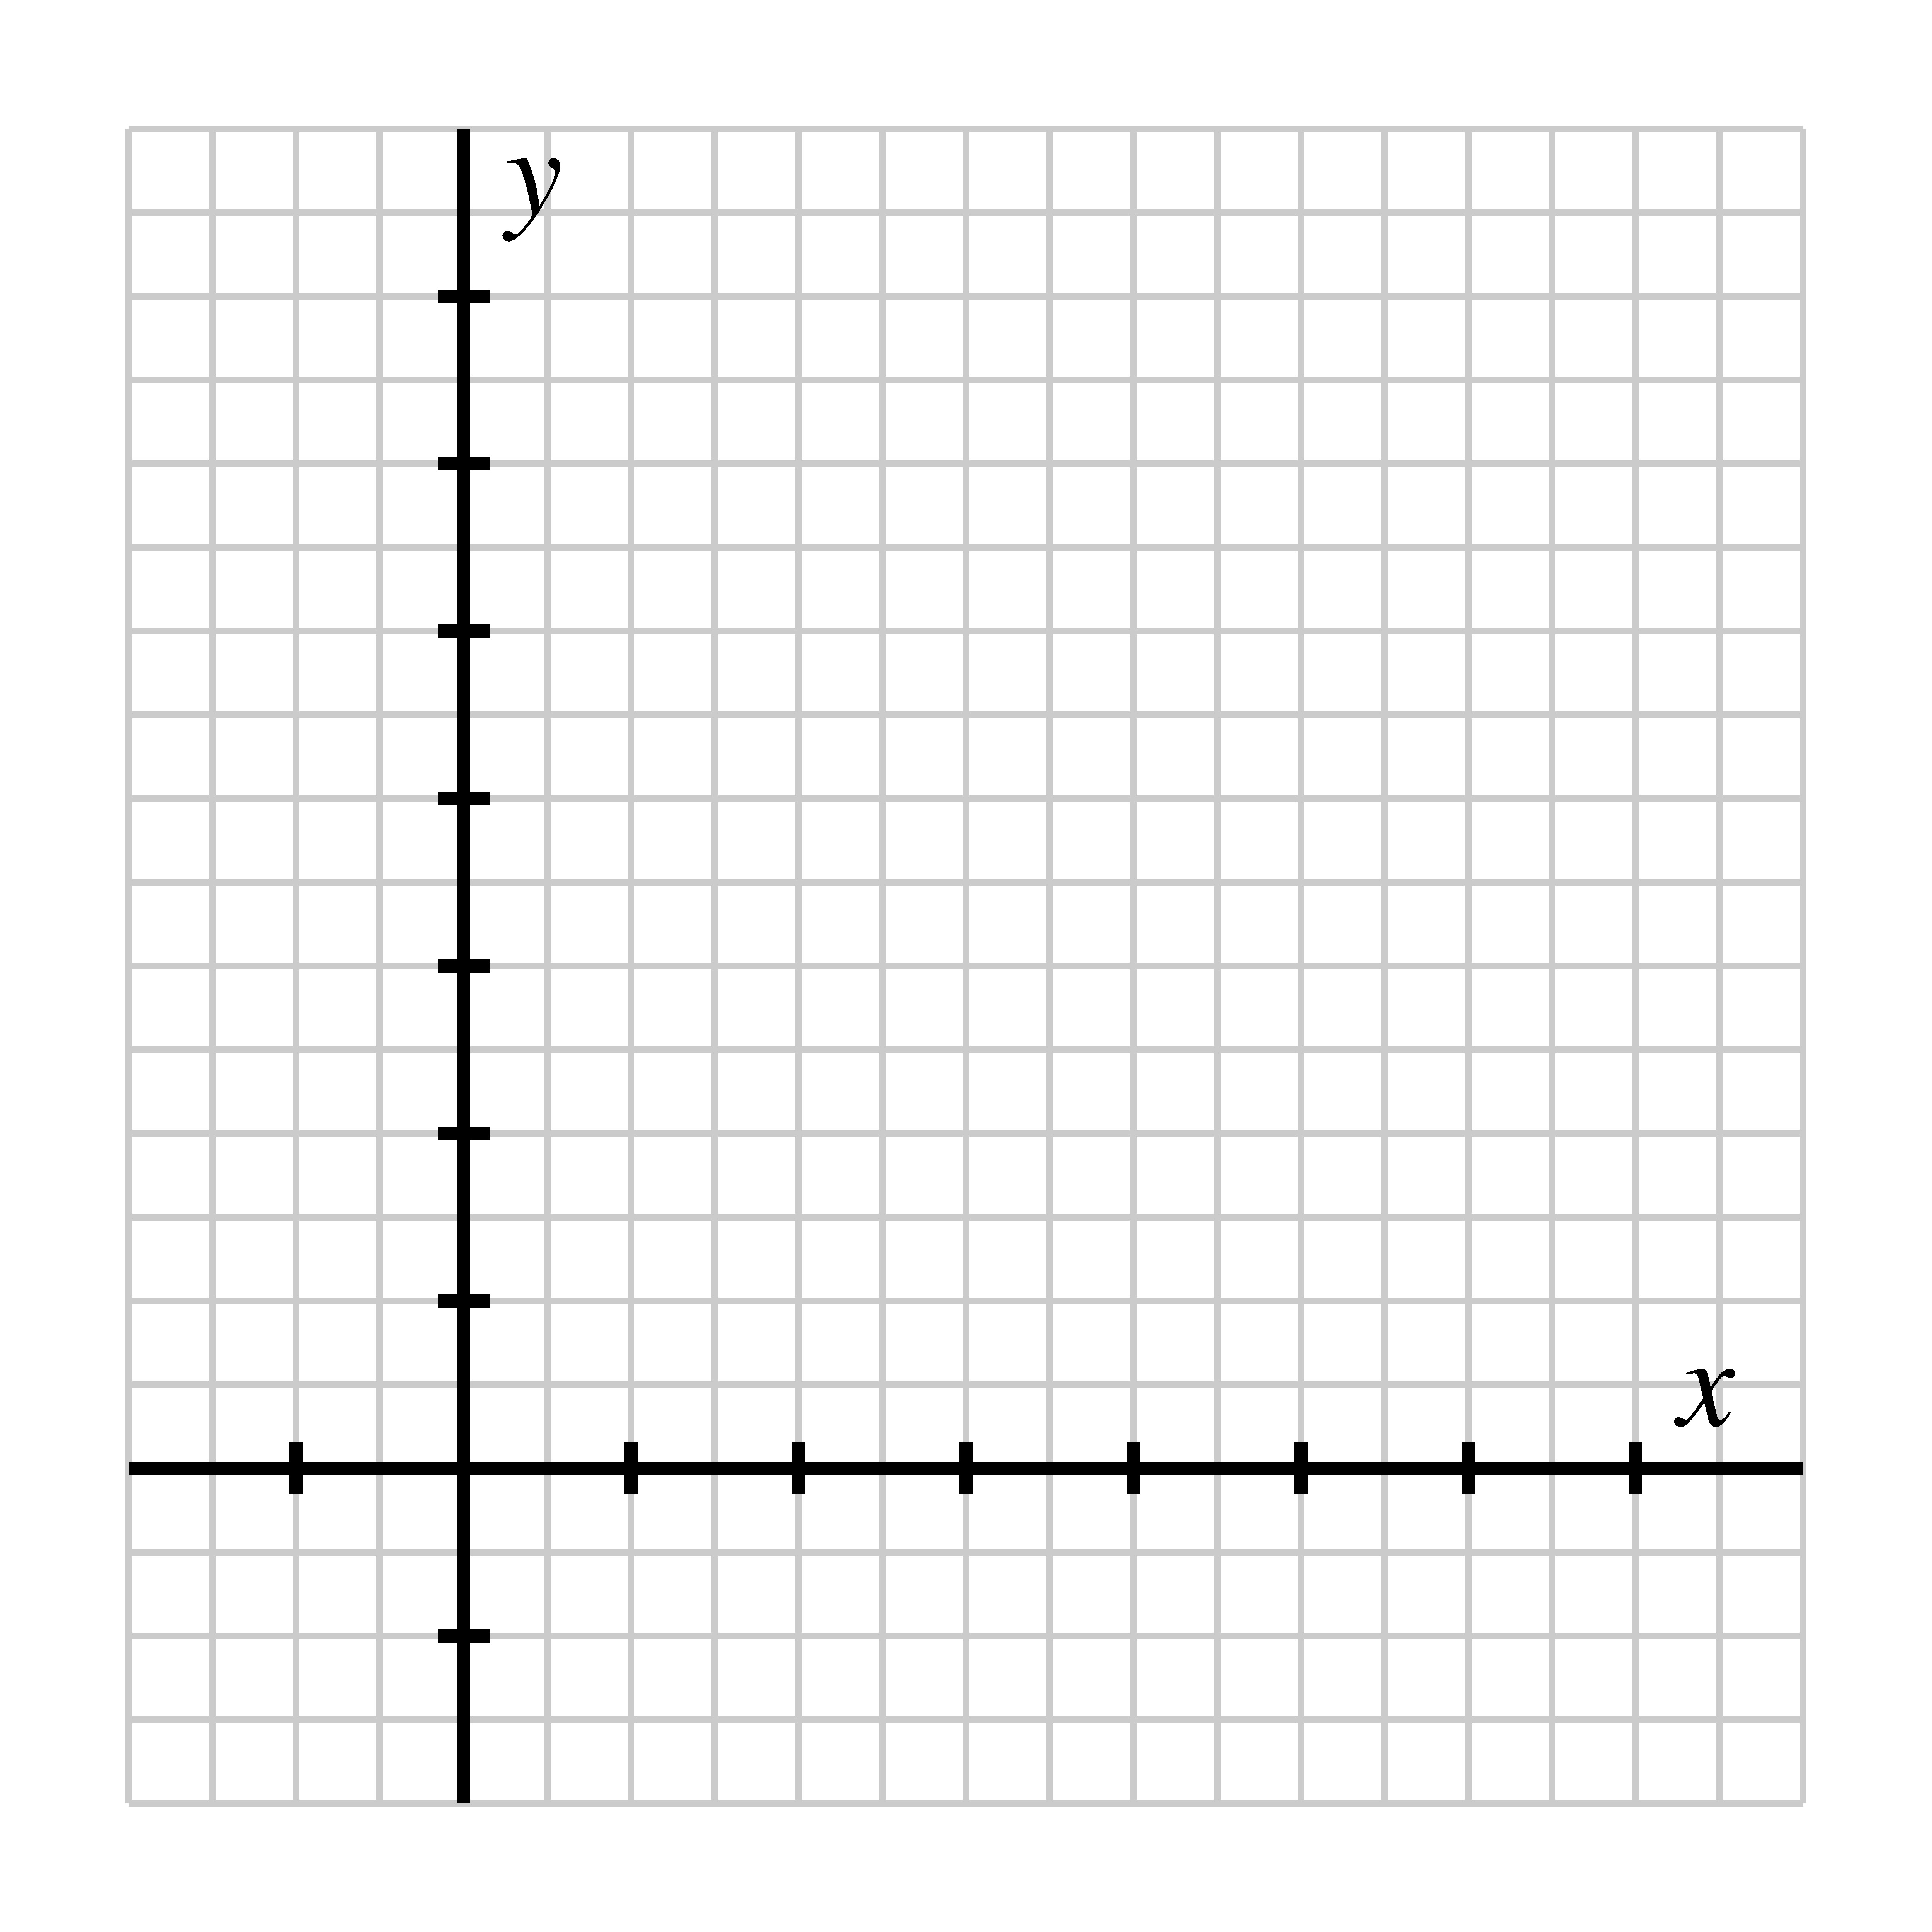
\includegraphics[width=.4\textwidth]{functions-y-x-blank-axes.jpg}
	}\\
	\end{array}
	$
	\end{center}


\item $h$ is a function defined on $[-1,7]$ such that $h(2) = 5$, $h(4) = 3$ and $\av_{[2,4]} = -2$.

	\begin{center}
	$
	\begin{array}{ccc}
	{
	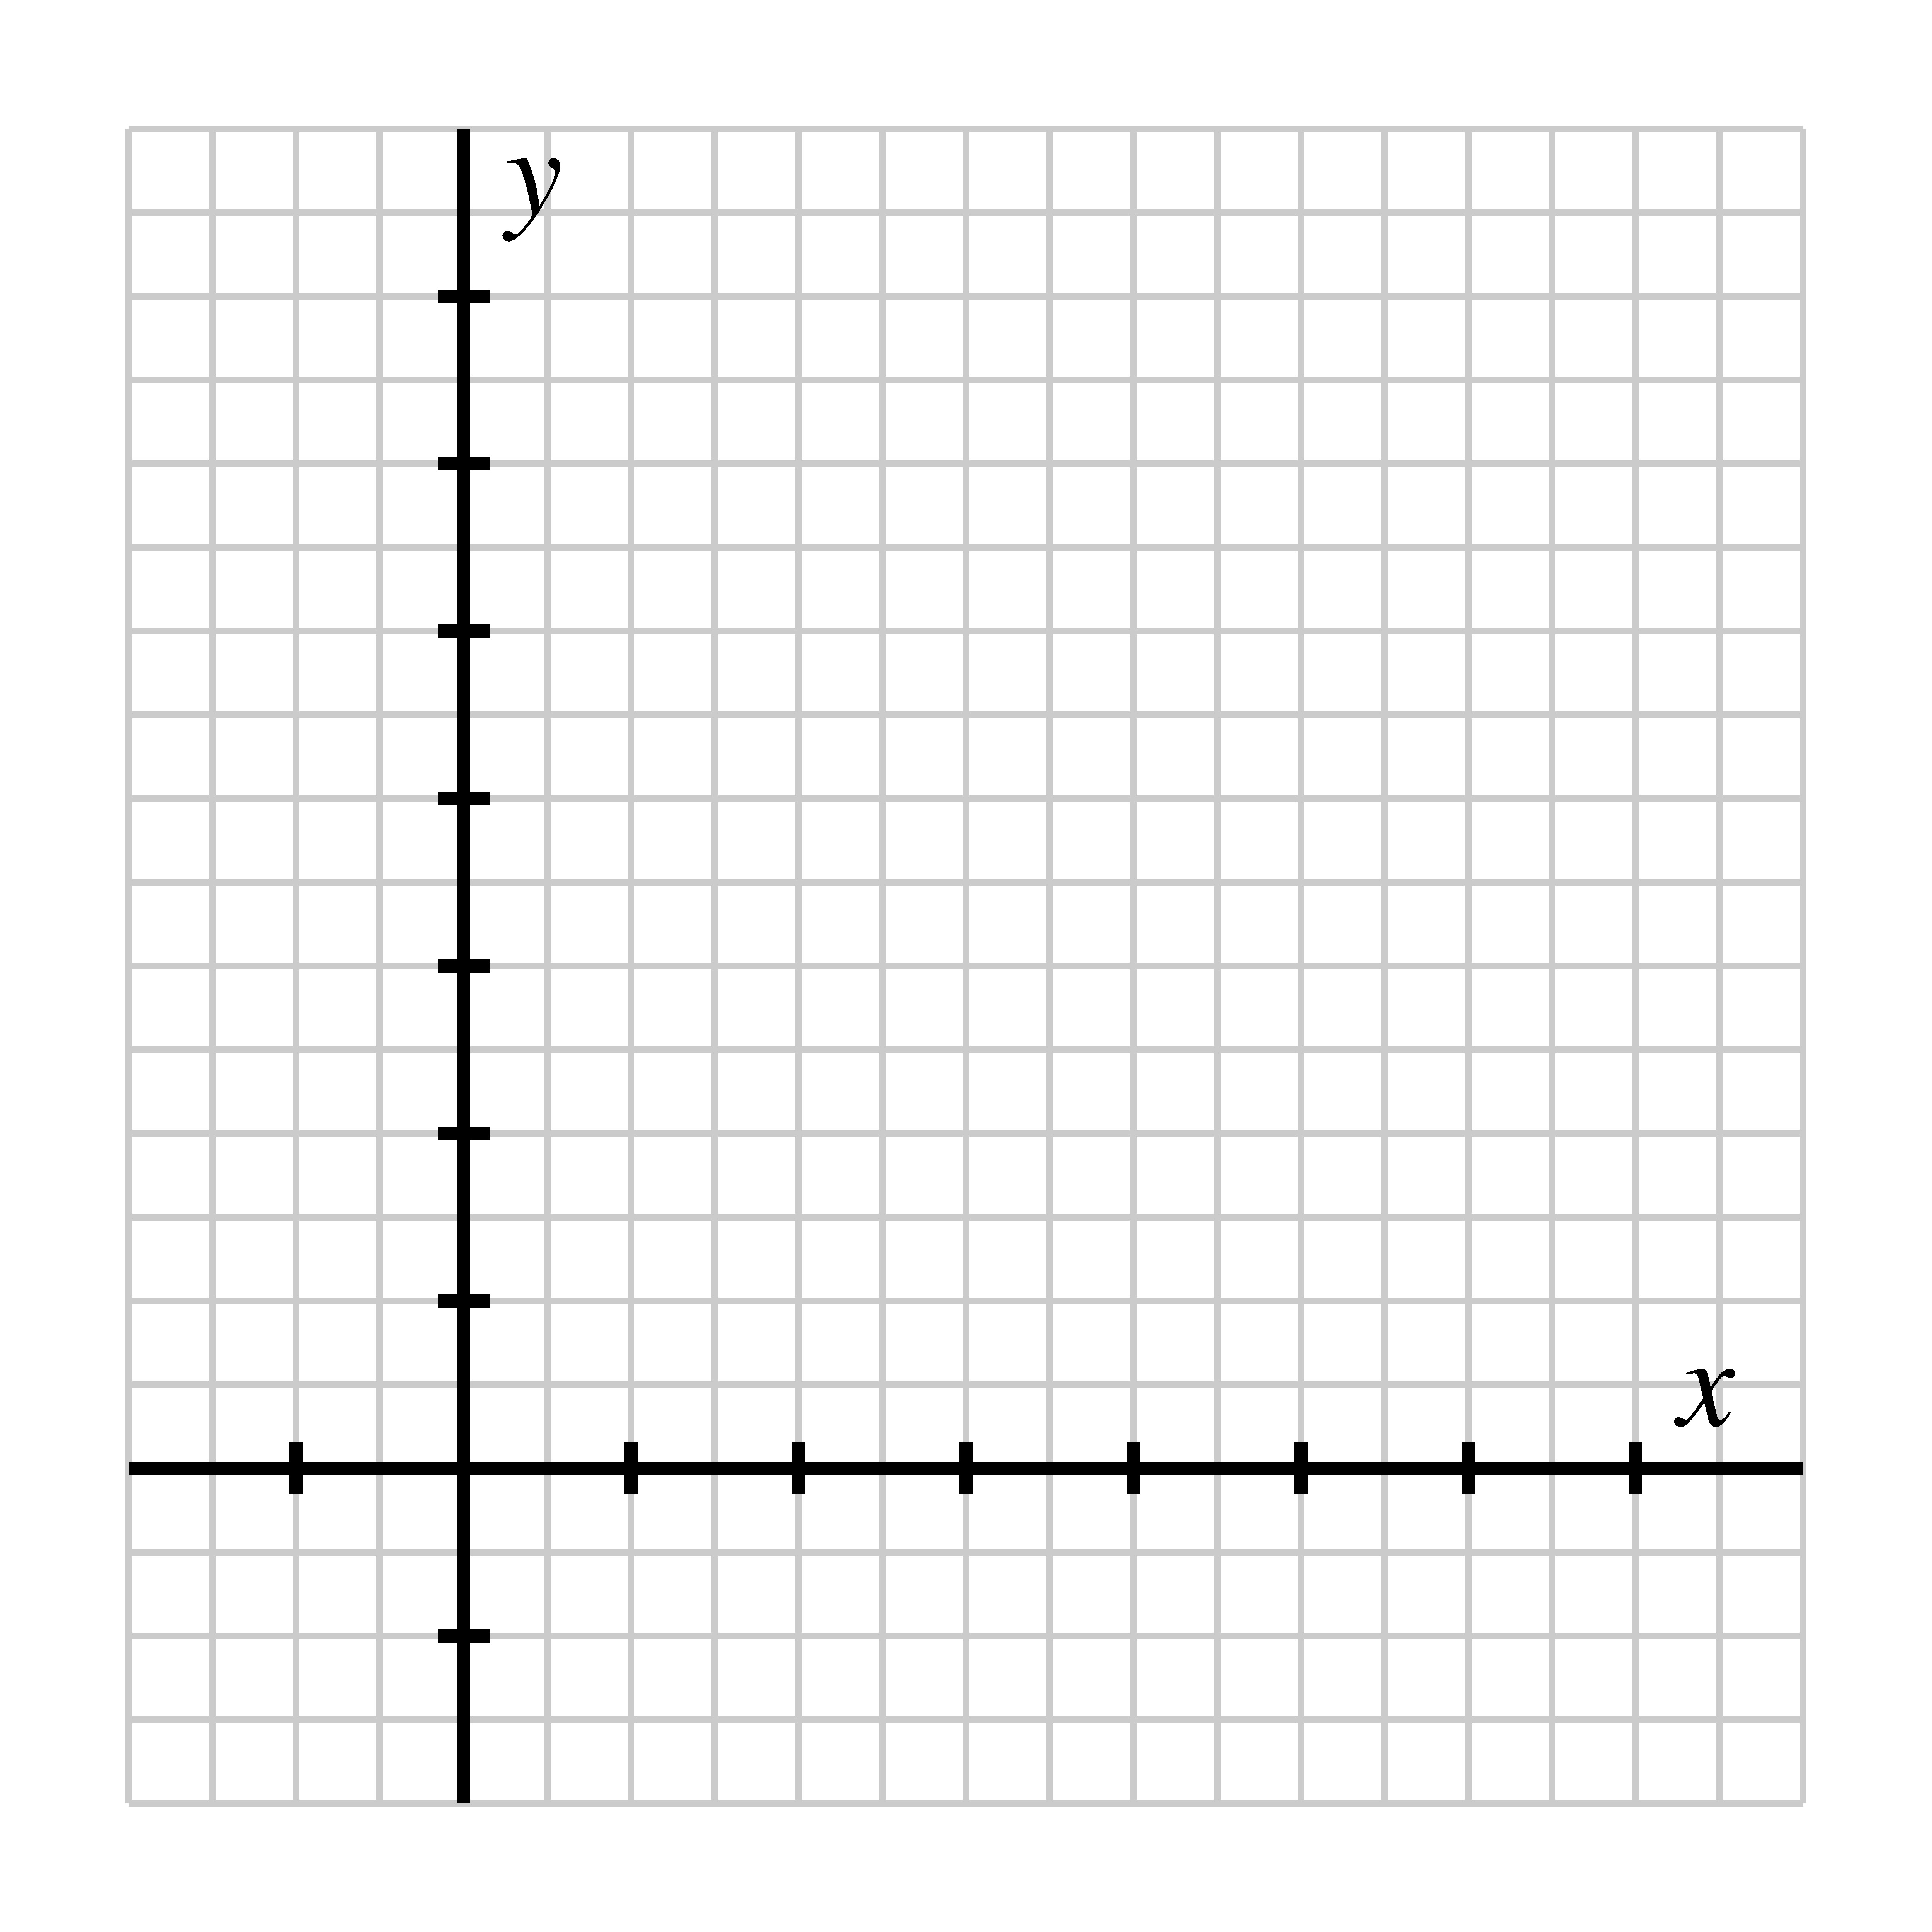
\includegraphics[width=.4\textwidth]{functions-y-x-blank-axes.jpg}
	}&&
	{
	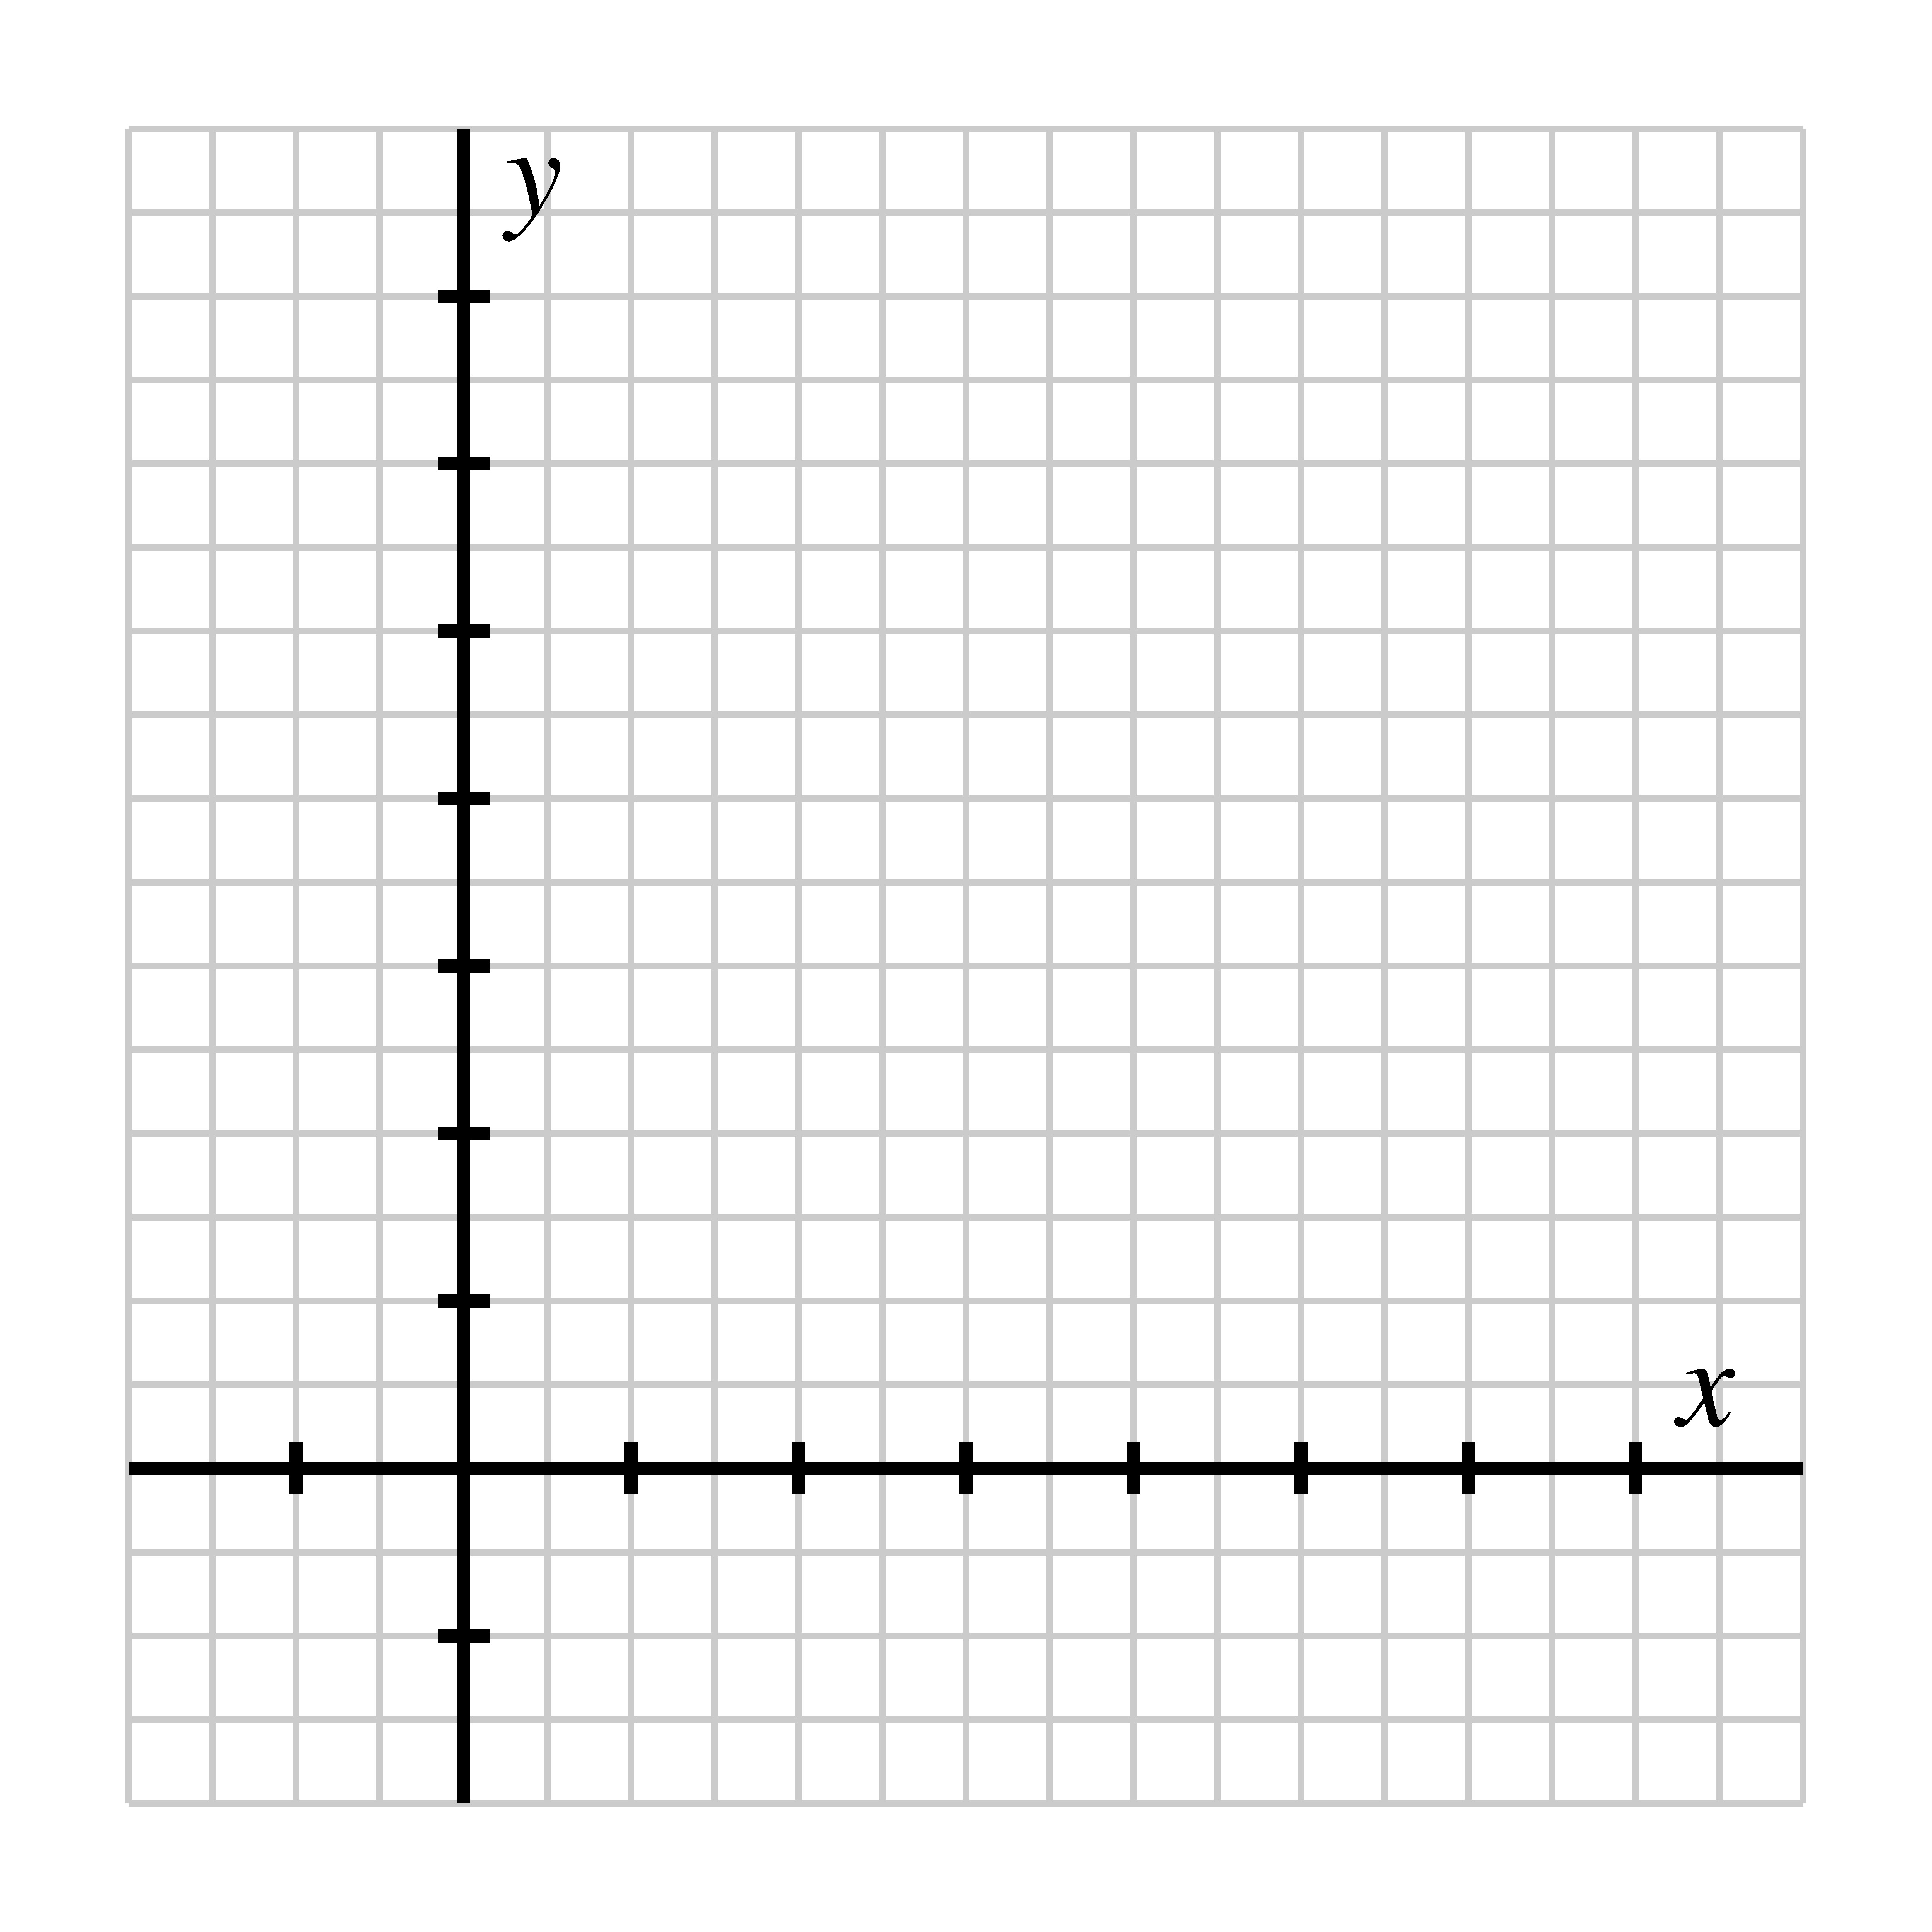
\includegraphics[width=.4\textwidth]{functions-y-x-blank-axes.jpg}
	}\\
	\end{array}
	$
	\end{center}

\end{enumerate}
\end{exploration}

\begin{summary}\begin{itemize}
\item For a function $f$ defined on an interval $[a,b]$, the average rate of change of $f$ on $[a,b]$ is the quantity%
\begin{equation*}
\av_{[a,b]} = \frac{f(b) - f(a)}{b-a}\text{.}
\end{equation*}
\item The value of $\av_{[a,b]} = \frac{f(b) - f(a)}{b-a}$ tells us how much the function rises or falls, on average, for each additional unit we move to the right on the graph.  For instance, if $\av_{[3,7]} = 0.75$, this means that for additional $1$-unit increase in the value of $x$ on the interval $[3,7]$, the function increases, on average, by $0.75$ units.  In applied settings, the units of $\av_{[a,b]}$ are ``units of output per unit of input''.
\item The value of $\av_{[a,b]} = \frac{f(b) - f(a)}{b-a}$ is also the slope of the line that passes through the points $(a,f(a))$ and $(b,f(b))$ on the graph of $f$, as shown in the graph below.
\begin{image}
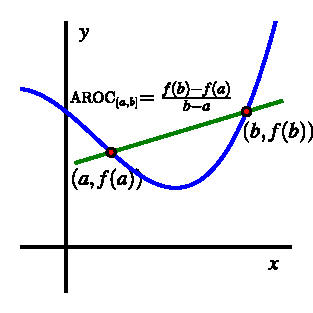
\includegraphics{aroc-f-x-defn.pdf}
\end{image}

\item This line passing through these two points $(a,f(a))$ and $(b,f(b))$, is called a secant line to the graph, and its slope is equal to the average rate of change of the function on the interval $[a,b]$.

\end{itemize}\end{summary}

\end{document}
